\documentclass[
    a4paper, aps, twocolumn, floatfix, superscriptaddress,
    nofootinbib]{revtex4-1}

% It's nice to be able to write your own name
\usepackage[T1]{fontenc}
% Automatic clickable links
\usepackage{hyperref}
% SI-units
\usepackage{siunitx}
% Enhanced math formatting
\usepackage{amsmath}
% Extended math symbols
\usepackage{amssymb}
% Include proof environment
\usepackage{amsthm}
% Import physics package to include bra-ket
\usepackage{physics}
\usepackage{enumerate}
% Import the tensor package for tensors
\usepackage{tensor}
% Include dod and dpd fracs
\usepackage{commath}
% Include font for the identity operator
\usepackage{dsfont}
% Include Tikz
\usepackage{tikz}
% Tikz add-on
\usetikzlibrary{shapes,arrows}
\usetikzlibrary{positioning}
% Several figures in the same figure
\usepackage{subfig}
% Appendix
\usepackage[toc, page]{appendix}

% Macro for latin-letter vectors
\newcommand{\vf}{\mathbf}
% Macro for greek-letter vectors
\newcommand{\vfg}{\boldsymbol}

% Fast macro for real-numbers R
\newcommand{\R}{\mathbb{R}}
% Fast macro for complex-numbers C
\newcommand{\C}{\mathbb{C}}
% Fast macro for polynomial room P
\renewcommand{\P}{\mathbb{P}}
% New command for the identity operator
\newcommand{\1}{\mathds{1}}
% New command for the Lagrangian density
\newcommand{\cL}{\mathcal{L}}
% New command for the Hamiltonian density
\newcommand{\cH}{\mathcal{H}}
% Fast macro for partial differential tensors
\newcommand{\tpl}[1]{\tensor{\partial}{_#1}} % Lower
\newcommand{\tpu}[1]{\tensor{\partial}{^#1}} % Upper
% Fast macro for tensors
\newcommand{\te}[1]{\tensor{#1}}
% Fast macro for commutation and anti-commutation relations
\newcommand{\com}[2]{\left[#1, #2\right]}
\newcommand{\acom}[2]{\left\{#1, #2\right\}}

% Macros for writing auto-sized paranthesis, brackets and braces
\newcommand{\para}[1]{\left(#1\right)}
\newcommand{\brak}[1]{\left[#1\right]}
\newcommand{\brac}[1]{\left\{#1\right\}}

% Macro for creating orbital bra-ket's, i.e., bra-ket with paranthesis edges
\newcommand{\obra}[1]{( #1 \lvert}
\newcommand{\oket}[1]{\rvert #1 )}
\newcommand{\obraket}[2]{( #1 \lvert #2 )}

% Macro for expectation value
\newcommand{\expv}[1]{\langle #1 \rangle}

\newcommand{\half}{\frac{1}{2}}




\begin{document}

\title{Variational Monte Carlo on Bosonic Systems}
\author{Winther-Larsen, Sebastian Gregorius}
\homepage[Project code: ]{https://github.com/Schoyen/FYS4411}
\affiliation{University of Oslo}
\author{Schøyen, Øyvind Sigmundson}
\homepage[Project code: ]{https://github.com/Schoyen/FYS4411}
\affiliation{University of Oslo}
\date{\today}

\begin{abstract}
    In this project we use Quantum Variational Monte Carlo on a toy model of a
    bosonic gas  in an elliptic trap. The framework we have built is first
    tested against analytic solutions of simple non-interacting systems. From
    there the system is extended to include perturbed harmonic oscillator traps
    and particle interaction. We compute one-body densities for the interacting
    case and discuss why this tool is important and how our toy model has
    similar attributes to real-world systems.
\end{abstract}

\maketitle
\tableofcontents


\section{Introduction}
    We will in this project study the Variational Monte Carlo method, and use it
    to evaluate the ground state energy of a trapped, hard sphere Bose gas.

    By building up an increasingly intricate system we eloquently illustrate the
    strength of the Variational Monte Carlo methods. Any Monte Carlo method
    draws on the fact that the computer will not complain when being tasked to
    perform a very similar task up to several million times in rapid succession.
    Monte Carlo methods is in essence a series of guesses where the current
    guess is only a minor alteration of the one prior to it. The trick lies in
    only accepting the subsequent guesses that improves upon our configuration
    up to a certain likelihood.

    The method we have employed is called a \emph{Variational} Monte Carlo
    method, because we make an educated guess at a trial wavefunction which we
    allow certain degrees of freedom called \emph{variational parameters}. We
    shall see that the system converges to a proper \footnote{Global, as far as
    we can tell.} minimum for only a certain set of parameters.

    First, we provide the theoretical foundation for the Variational Monte Carlo
    method. This includes explaining how Monte Carlo integration works, and
    introducing the important quantities \emph{local energy}, \emph{drift force}
    and \emph{one-body densities}.

    Second, we outline in more detailed algebra the nature of the systems we
    will be studying. For the non-interacting system we are able to derive an
    exact variational energy to which we can compare the results from our
    simulations. We furthermore give a description of an interacting system
    implemented as if each particle is a hard sphere.

    Third, we provide a thorough description of algorithms and statistical
    methods employed in this study. Here we introduce the Metropolis-Hastings
    algorithm. This algorithm can by a deft trick be expanded with the method of
    \emph{importance sampling} yielding a more intelligent choice for the next
    step in the Monte Carlo cycling.  The main point of note with regards to the
    statistical analysis is that the data generated by the Monte Carlo cycling
    is autocorrelated and computation of variance must be done with the
    \emph{blocking method} for time series data.  As an automated way of finding
    the optimal variational parameter, we sketch out the method of
    \emph{gradient descent}.

    Fourth, we put the machinery described in the previous sections to work. We
    test against the actual values in a non-interacting system before analyzing
    the more interesting perturbed-trap system with interacting particles.

    Lastly, we highlight interesting aspects of this study in a discussion of
    the results before ending on some summary remarks.

\section{Variational Monte Carlo}
    The variational principle states that for a given \emph{trial wavefunction},
    $\ket{\Psi_T}$, the expectation value of the Hamiltonian, $H$, will be an
    upper bound to the ground state energy, $E_0$ of the system.
    \begin{align}
        E_0 \leq E
        = \frac{\bra{\Psi_T}H\ket{\Psi_T}}{\bra{\Psi_T}\ket{\Psi_T}},
    \end{align}
    The complicated part of the variational principle is finding the trial
    wavefunction that minimizes the energy. The strength in this method lies in
    introducing variational parameters in the trial wavefunction. Using these as
    degrees of freedom we can minimize the energy with respect to these in order
    to find an infimum to the ground state energy for the given trial
    wavefunction and Hamiltonian. For a select few systems we can calculate this
    analytically, but for the interesting systems we quickly hit an intractable
    wall as the systems become analytically unsolvable. To get around this we
    try to calculate the energy for a given Hamiltonian and a trial wavefunction
    for different variational parameters numerically.


    To determine if we have located a minimum we can use the variance of the
    variational energy.
    \begin{align}
        \sigma^2
        &=
        \frac{
            \bra{\Psi_T}H^2\ket{\Psi_T}
        }{
            \bra{\Psi_T}\ket{\Psi_T}
        }
        - \para{
            \frac{
                \bra{\Psi_T}H\ket{\Psi_T}
            }{
                \bra{\Psi_T}\ket{\Psi_T}
            }
        }^2.
    \end{align}
    If we have found the "true" trial wavefunction $\ket{\Psi_T}$ with the
    correct variational parameters, i.e., the eigenfunction to the Hamiltonian
    we get $\sigma^2 = 0$. We are thus interested in trying to find the
    variational parameters in the trial wavefunction that minimizes the
    variance.

    \subsection{Monte Carlo integration}
        Unfortunately the evaluation of the expectation value of the energy for
        a given trial wavefunction involves a large integral.
        \begin{align}
            E
            &= \frac{\bra{\Psi_T}H\ket{\Psi_T}}{\bra{\Psi_T}\ket{\Psi_T}}
            =
            \frac{\int\dd\vf{r}\Psi_T^{*}(\vf{r})H\Psi_T(\vf{r})}
            {\int\dd\vf{r}|\Psi_T|^2},
        \end{align}
        where $\vf{r} = (\vf{r}_1, \vf{r}_2, \dots \vf{r}_N)$ are the
        positions\footnote{This can include both spatial and spin parts, but we
        will in the remainder of this project ignore spin.} of the particles
        contained in the system.

        To get around\footnote{Not exactly \emph{get around} per se. We still
        have to evaluate the integral, but we make the problem solvable at all.}
        the trouble of evaluating the multidimensional-integral we employ the
        method of Monte Carlo integration. This consists of approximating an
        integral of the expectation value of a certain quantitity by a sum.
        \begin{align}
            \expval{x}
            &=
            \int_{\mathbb{R}}xp(x)\dd x
            \approx
            \frac{1}{N}\sum_{i = 1}^N x_ip(x_i),
        \end{align}
        where $x$ is a random variable with a probability density function
        $p(x)$ and $\{x_i\}$ for $i \in \{1, \dots, N\}$ is the set of drawn
        random variables. Here $N$ is the number of Monte Carlo samples chosen
        to approximate the integral. By the law of large numbers we expect that
        \begin{align}
            \lim_{N \to \infty}\frac{1}{N}\sum_{i = 1}^N x_ip(x_i)
            = \expval{x}.
        \end{align}

        For us to be able to take Monte Carlo integration to the quantum realm
        we have to construct a probability density function from the
        wavefunction. Luckily the wavefunction squared is just such a quantity.
        Given a normalized wavefunction $\ket{\psi}$ we can compute the
        expectation value of a quantum operator $\mathcal{O}$ using Monte
        Carlo integration.
        \begin{align}
            \expval{\mathcal{O}}
            &= \bra{\psi}\mathcal{O}\ket{\psi}
            =
            \int\dd\vf{r}
            \psi^{*}(\vf{r})\mathcal{O}\psi(\vf{r})
            \\
            &=
            \int\dd\vf{r}
            |\psi(\vf{r})|^2
            \frac{\mathcal{O}\psi(\vf{r})}{\psi(\vf{r})},
        \end{align}
        where we have multiplied and divided by the wavefunction. We now define
        the probability density function, $p(\vf{r})$, as
        \begin{align}
            p(\vf{r}) \equiv |\psi(\vf{r})|^2,
        \end{align}
        and the local quantum operator
        \begin{align}
            \mathcal{O}_L(\vf{r})
            &\equiv \frac{\mathcal{O}\psi(\vf{r})}{\psi(\vf{r})}.
        \end{align}
        We see that if the chosen wavefunction is an eigenstate of the quantum
        operator, the local quantum operator becomes a constant.  We can thus
        approximate the expecatation value of the quantum operator using Monte
        Carlo integration.
        \begin{align}
            \expval{O}
            &=
            \int\dd\vf{r}
            p(\vf{r})
            \mathcal{O}_L(\vf{r})
            \approx
            \frac{1}{N}\sum_{i = 1}^N
            p(\vf{r}_i)\mathcal{O}_L(\vf{r}_i).
        \end{align}
        In the case of a non-normalized wavefunction we need to divide by a
        normalization factor in the probability density function.


    \subsection{Local energy}
        As is mostly the case in physics, the quantity we are looking for is the
        energy. We therefore define the \emph{local energy} by
        \begin{align}
            E_L(\vf{r})
            &= \frac{H\Psi_T(\vf{r})}{\Psi_T(\vf{r})}.
        \end{align}
        The energy of the system is thus found by computing the expectation
        value of the local energy.
        \begin{align}
            \expval{E_L}
            =
            \frac{
                \int\dd \vf{r}|\Psi_T(\vf{r})|^2 E_L(\vf{r})
            }{
                \int\dd \vf{r}|\Psi_T(\vf{r})|^2
            }
            \approx
            \frac{1}{N}\sum_{i = 1}^N
            p(\vf{r}_i)E_L(\vf{r}_i).
        \end{align}
        To determine if we have found a minimum we compute the variance of the
        expectation value of the local energy.
        \begin{align}
            \sigma^2 = \langle E_L^2\rangle - \expval{E_L}^2.
        \end{align}
        One of the most computationally intensive parts of the Variational Monte
        Carlo algorithm will be to compute $E_L$. We will therefore find an
        analytical expression for $E_L$ in terms of the trial wavefunctions and
        the system we are exploring.

    \subsection{The drift force}
        A disadvantage in the use of the brute force Metropolis-Hastings
        algorithm is that we might be spending much computational resources in
        an uninteresting part of configuration space. To make smarter moves we
        will add importance sampling (which will be discussed in due time) to
        the algorithm. This alteration of the algorithm needs a new quantity
        called the \emph{drift force} of the system\footnote{Also known as the
        \emph{quantum force}.}.
        \begin{align}
            \vf{F}(\vf{r})
            &=
            \sum_{k = 1}^N
            \vf{F}_k(\vf{r})
            =
            \sum_{k = 1}^N
            \frac{2\nabla_k\Psi_T(\vf{r})}{\Psi_T(\vf{r})}.
            \label{eq:drift_force}
        \end{align}
        Using the drift force we are able to move towards more interesting parts
        of configuration space as we are following the gradient of the
        wavefunction. We will mainly be interested in the drift force of a
        single particle $k$ as the Monte Carlo sampling involves choosing a
        single particle at a time.

    \subsection{One-Body Densities}
        In order to make some conclusion towards where the particles in our
        systems are most prone to exist, we need a good way to visualise our
        wavefunctions. If we are to visualize the combined wavefunction of two
        three-dimensional particles we need four dimensions per particle and can
        subtract one dimension as we look at a single probability density
        yielding a grand total of seven dimensions. The fact that we will be
        studying systems of up to $N = 500$ particles only adds to the headache.
        We therefore introduce the single-particle density function, or
        \emph{one-body density} $\rho(\vf{r})$. The one-body density is defined
        by the integral over all coordinates except
        one\cite{kristiansen2017time},
        \begin{align}
            \rho(\vf{r}_1)
            \equiv
            \int \dd\vf{r}_2 \dots \dd\vf{r}_N
            \abs{\Psi(\vf{r}_1, \dots, \vf{r}_N)}^2.
        \end{align}
        The one-body density represents the distribution of all the particles in
        the system. Furthermore, $\rho(\vf{r}_1)\dd\vf{r}_1$ will yield the
        probability of finding any particle within the volume element
        $\dd\vf{r}_1$. By convention the one-body density should be normalized
        such that the following relation holds,
        \begin{align}
            N = \int \rho(\vf{r}_1)\dd\vf{r}_1.
        \end{align}
        In other words, the integral over the entire volume in
        $\vf{r}_1$-direction gives us the total number of particles in our
        system. This can be a bit odd at first sight as we are used to getting
        unity when we integrate over the entire probability
        density.\cite{hogberget2013quantum}

        It is best to think of the one-body density as the multivariate
        probability density for the entire system collapsed down to one
        coordinate in a representation than looks very familiar to every
        physicist with a basic knowledge of quantum mechanics.

\section{Systems}
    To model the trapped bosonic gas particles we use the potential
    \begin{align}
        v(\vf{r})
        &=
        \begin{cases}
            \half m\omega^2r^2 & (\text{S}), \\
            \half m \bigl[
                \omega^2(x^2 + y^2) + \omega_z^2z^2
            \bigr] & (\text{E}),
        \end{cases}
    \end{align}
    where we can choose between a spherical (S) or an elliptical (E) harmonic
    oscillator trap. The full Hamiltonian of the system is given by
    \begin{align}
        H = \sum_{i = 1}^{N}h(\vf{r}_i) + \sum_{i < j}^{N}w(\vf{r}_i, \vf{r}_j),
    \end{align}
    where the single particle one-body operator, $h(\vf{r}_i)$, is given by
    \begin{align}
        h(\vf{r}_i) = -\frac{\hbar^2}{2m}\nabla_i^2
        + v(\vf{r}_i),
    \end{align}
    for equal masses. The two-body interaction operator, $w(\vf{r}_i,
    \vf{r}_j)$, is
    \begin{align}
        w(\vf{r}_i, \vf{r}_j)
        = \begin{cases}
            \infty & |\vf{r}_i - \vf{r}_j| \leq a, \\
            0 & |\vf{r}_i - \vf{r}_j| > a,
        \end{cases}
        \label{eq:two-body_interaction}
    \end{align}
    where $a$ is the hard sphere of the particle.  The trial wavefunction we
    will be looking at is given by
    \begin{align}
        \Psi_T(\vf{r})
        &= \Phi_T(\vf{r})
        J(\vf{r}),
        %\\
        %&= \Biggl(
        %    \prod_{i = 1}^N g(\alpha, \beta, \vf{r}_i)
        %\Biggr)
        %\prod_{j < k}^N f(a, \vf{r}_j, \vf{r}_k),
        \label{eq:initial_trial_wavefunction}
    \end{align}
    where $\vf{r} = (\vf{r}_1, \dots, \vf{r}_N)$. The Slater permanent,
    $\Phi_T(\vf{r})$, is given by the $N$ first single-particle functions
    \begin{align}
        \Phi_T(\vf{r})
        &=
        \prod_{i = 1}^N \phi(\vf{r}_i)
        = \prod_{i = 1}^N\exp\bigl[
            -\alpha(x_i^2 + y_i^2 + \beta z_i^2)
        \bigr].
    \end{align}
    Here $\alpha$ is the variational parameter of the trial
    wavefunction.\footnote{We can also treat $\beta$ as a variational parameter,
    but we will in this project limit ourselves to a single variational
    parameter, i.e., $\alpha$.} The Jastrow factor, $J(\vf{r})$ contributes with
    correlations between the particles and is represented as
    \begin{align}
        J(\vf{r})
        &=
        \prod_{j < k}^N f(a, \vf{r}_j, \vf{r}_k),
    \end{align}
    where the correlation wavefunctions are given by
    \begin{align}
        f(a, \vf{r}_j, \vf{r}_k)
        &=
        \begin{cases}
            0 & |\vf{r}_j - \vf{r}_k| \leq a, \\
            \Bigl(
                1 - \frac{a}{|\vf{r}_j - \vf{r}_k|}
            \Bigr) & |\vf{r}_j - \vf{r}_k| > a.
        \end{cases}
        \label{eq:correlation_wavefunction}
    \end{align}
    We will for brevity define the notation
    \begin{gather}
        \phi_i \equiv \phi(\vf{r}_i),
        \\
        r_{jk} \equiv \abs{\vf{r}_j - \vf{r}_k}.
    \end{gather}
    In practice \autoref{eq:two-body_interaction} is
    unnecessary as the situtation where $r_{jk} \leq a$ automatically yields a
    probability density of zero from \autoref{eq:correlation_wavefunction} thus
    rejecting the state completely.

    \subsection{Non-interacting harmonic oscillators}
        We start by looking at a simple system of non-interacting harmonic
        oscillators, where $a = 0$ and $\beta = 1$. This means that there is no
        hard-shell interaction between the particles and that we use a spherical
        potential trap.  We thus get the trial  wavefunction
        \begin{align}
            \Psi_T(\vf{r})
            = \Phi_T(\vf{r})
            = \prod_{i = 1}^N \exp\para{
                -\alpha |\vf{r}_i|^2
            }.
            \label{eq:trial_simple_gaussian}
        \end{align}
        As $a = 0$ the interaction term, $w(\vf{r}_i, \vf{r}_j)$, vanishes and
        the Hamiltonian is given by (in the spherical case)
        \begin{align}
            H &= \sum_{i = 1}^N h(\vf{r}_i)
            = \sum_{i = 1}^N \Biggl(
                -\frac{\hbar^2}{2m}\nabla_i^2
                + \half m \omega^2 r_i^2
            \Biggr).
        \end{align}
        To find the drift force and the local energy we have to compute the
        gradient and the Laplacian of the trial wavefunction. The gradient is
        given by
        \begin{align}
            \nabla_k\Psi_T(\vf{r})
            &= -2\alpha \vf{r}_k\Psi_T(\vf{r}),
        \end{align}
        whereas the Laplacian yields
        \begin{align}
            \nabla^2_k\Psi_T(\vf{r})
            &= \big(-2d\alpha + 4\alpha^2 r_k^2\bigr)\Psi_T(\vf{r}).
            \label{eq:laplacian_simple_gaussian}
        \end{align}
        Here $d$ is the dimensionality of the problem determined by $\vf{r}_k
        \in \mathbb{R}^d$. We can thus use the gradient to find an expression
        for the drift force for particle $k$.
        \begin{align}
            \vf{F}_k(\vf{r})
            &= -4\alpha\vf{r}_k.
        \end{align}
        Using the Laplacian we can compute the kinetic term in the expression
        for the local energy. We get
        \begin{align}
            E_L(\vf{r})
            &=
            \sum_{i = 1}^N
            \Biggl(
                -\frac{\hbar^2}{2m}
                \bigl[
                    -2d\alpha + 4\alpha^2 r_i^2
                \bigr]
                + \half m\omega^2 r_i^2
            \Biggr).
        \end{align}
        In natural units, $\hbar = c = 1$, and with the mass set to unity this
        reduces to
        \begin{align}
            E_L(\vf{r})
            &=
            \alpha dN
            + \biggl(
                \half\omega^2
                - 2\alpha^2
            \biggr)
            \sum_{i = 1}^N r_i^2.
            \label{eq:closed_form_natural_units_local_energy}
        \end{align}
        It is worth noting that for $\alpha = \omega/2$\footnote{Note that
        $\alpha$ is required to be positive.} we get a stable value for the
        local energy.
        \begin{align}
            E_L(\vf{r}; \alpha = \omega/2)
            &\equiv
            E_L
            =
            \frac{\omega d N}{2},
            \label{eq:minimum_energy_simple}
        \end{align}
        which turns out to be the exact minimum for the ground state energy of
        this system as we shall see.

        \subsubsection{Exact variational energy}
            As the system is non-interacting and consisting of Gaussians we can
            find an expression for the exact energy as a function of the
            variational parameter $\alpha$, i.e.,
            \begin{align}
                E(\alpha)
                &=
                \frac{\bra{\Psi_T}H\ket{\Psi_T}}{\bra{\Psi_T}\ket{\Psi_T}}
                =
                \left(
                    \frac{\hbar^2 \alpha}{2m}
                    + \frac{m\omega^2}{8\alpha}
                \right)dN.
                \label{eq:exact_energy}
            \end{align}
            By minimizing this expression with respect to $\alpha$ we get
            \begin{align}
                \dod[]{E(\alpha)}{\alpha} = 0
                \implies
                \alpha_0 = \frac{m\omega}{2\hbar},
            \end{align}
            which in natural units reduces to $\alpha_0 = \omega/2$. The energy
            at this value of $\alpha$ (in natural units) is then
            \begin{align}
                E(\alpha_0)
                &=
                \frac{\omega dN}{2},
            \end{align}
            in perfect accordance with \autoref{eq:minimum_energy_simple} which
            yields high hopes for the latter equation and the expected minimum.


    \subsection{Interacting hard sphere bosons}
        Moving to the full elliptical system for $\beta \neq 1$ and setting $a
        \neq 0$ we use the trial wavefunction from
        \autoref{eq:initial_trial_wavefunction}. We rewrite the Jastrow factor
        to
        \begin{align}
            J(\vf{r})
            &=
            \exp\para{
                \sum_{j < l}^N u(r_{jl})
            },
        \end{align}
        where
        \begin{align}
            u(r_{jk})
            = \ln\bigl[f(a, \vf{r}_j, \vf{r}_k)\bigr]
            \equiv u_{jk}
        \end{align}
        The drift force for particle $k$ in this system becomes
        \begin{align}
            \vf{F}_k(\vf{r})
            &=
            2\Biggl(
                \frac{\nabla_k\phi_k}{\phi_k}
                + \sum_{m \neq k}^N
                \nabla_k u_{km}
            \Biggr).
        \end{align}
        The Laplacian of particle $k$ divided by the trial wavefunction is then
        \begin{widetext}
            \begin{align}
                \frac{\nabla_k^2\Psi_T(\vf{r})}{\Psi_T(\vf{r})}
                &=
                \frac{\nabla_k^2\phi_k}{\phi_k}
                + 2\frac{\nabla_k\phi_k}{\phi_k}
                \sum_{m \neq k}^N
                \frac{\Delta\vf{r}_{km}}{r_{km}}
                \dpd[]{u_{km}}{r_{km}}
                + \sum_{m\neq k}^N
                \para{
                    \frac{d - 1}{r_{km}}\dpd[]{u_{km}}{r_{km}}
                    + \dpd[2]{u_{km}}{r_{km}}
                }
                +
                \para{
                    \sum_{m \neq k}^N
                    \frac{\Delta\vf{r}_{km}}{r_{km}}
                    \dpd[]{u_{km}}{r_{km}}
                }^2,
                \label{eq:laplacian_full_system}
            \end{align}
        \end{widetext}
        where $\Delta \vf{r}_{km} = \vf{r}_k - \vf{r}_m$ and $d$ is the
        dimensionality. Evaluating the gradient and the Laplacian of the single
        particle functions yields
        \begin{gather}
            \frac{\nabla_k\phi_k}{\phi_k}
            =
            -2\alpha
            (x_k\vf{e}_i + y_k\vf{e}_j + \beta z_k\vf{e}_k),
            \\
            \frac{\nabla_k^2\phi_k}{\phi_k}
            =
            -2\alpha
            \big(
                d - 1 + \beta
            \bigr)
            + 4\alpha^2
            \bigl(
                x_k^2 + y_k^2 + \beta^2z_k^2
            \bigr).
        \end{gather}
        Repeating this for the correlation functions yields
        \begin{align}
            \dpd[]{u_{km}}{r_{km}}
            &=
            \frac{a}{r_{km}(r_{km} - a)},
            \\
            \dpd[2]{u_{km}}{r_{km}}
            &= \frac{a^2 - 2ar_{km}}{r_{km}^2(r_{km} - a)^2}.
        \end{align}
        The local energy is thus
        \begin{align}
            E_L(\vf{r})
            &=
            \sum_{k = 1}^N
            \brac{
                -\frac{\hbar^2}{2m}
                \frac{\nabla_k^2\Psi_T(\vf{r})}{\Psi_T(\vf{r})}
                + v(\vf{r}_k)
            },
        \end{align}
        where the Laplacian is given by \autoref{eq:laplacian_full_system}.  We
        will avoid writing out the full expression for the local energy for this
        system due to the size of the equation.

        \subsubsection{Scaling the system}
            We now introduce a scaled distance $\vf{r}' = \vf{r}/a_{\text{ho}}$
            \cite{dubois2001bose}, where
            \begin{align}
                a_{\text{ho}}
                &=
                \sqrt{\frac{\hbar}{m\omega}}.
            \end{align}
            We can then rewrite the Hamiltonian for the elliptic potential in terms
            of this new distance. By doing a variable substitution for each
            direction in the Laplace operator we get
            \begin{align}
                \nabla_k^2
                &=
                \frac{1}{a_{\text{ho}}^2}{\nabla_k'}^2.
            \end{align}
            The one-body part of the Hamiltonian then yields
            \begin{align}
                H
                &=
                \sum_{k = 1}^N
                \brac{
                    -\frac{\hbar^2}{2m}\nabla_k^2
                    + \half m\brak{
                        \omega^2(x_k^2 + y_k^2)
                        + \omega_z^2 z_k^2
                    }
                }
                \\
                &=
                \frac{\hbar\omega}{2}
                \sum_{k = 1}^N
                \brac{
                    -{\nabla_k'}^2
                    +
                    \brak{
                        {x_k'}^2 + {y_k'}^2 + \lambda^2{z_k'}^2
                    }
                },
                \label{eq:scaled_hamiltonian}
            \end{align}
            where we have introduced the dimensionless frequency $\lambda =
            \omega_z/\omega$. The wavefunction does not need to be scaled as the
            exponentials are already dimensionless. We only need to use the
            scaled hard core radius $a' = a/a_{\text{ho}}$. We are interested in
            using the radius $a' = 0.0043$ as in the references
            \cite{dubois2001bose} and \cite{nilsen2005vortices}.


\section{Algorithms}
    In this project we rely on a Monte Carlo approach of random sampling to
    obtain numerical results.  We simulate random walks over a volume in order
    to find optimal parameters in our trial wavefunctions.  The most common of
    such methods, which we make use of herein, is the Metropolis-Hastings
    algorithm.

    \subsection{The Metropolis-Hastings Algorithm}
        The Metropolis-Hastings algorithm can in our particular situation be
        condensed down to the following steps:

        \begin{enumerate}
            \item The system is initialised by a certain number $N$ of randomly
                generated positions, $\vf{r} = (\vf{r}_1, \dots, \vf{r}_N)$,
                which represent the particles\footnote{Also known as
                \emph{random walkers}.}. This allows us to evaluate the
                wavefunction at these points and compute the local energy
                $E_L(\vf{r})$.

            \item The initial configuration is changed by setting a new position
                for one of these particles. The particle is picked at random and
                is only allowed to move a predetermined step length.


            \item A ratio, $q$, between the probability density of the new
                wavefunction and the previous probability density is computed.
                We accept the step if $q \geq 1$, else we accept the step with a
                probability $p$. The latter is done by drawing a random uniform
                number, $x \in [0, 1]$, and checking if $q > x$.  This
                transition probability decides if the particle move is rejected
                or accepted.

            \item If the particle movement is accepted we compute the local
                energy for the new system. If not, we reset the system to the
                previous state and reuse the last local energy.

            \item Accumulate the local energy. Repeat the steps until
                convergence is reached or a set number of iterations has been
                done. When finished divide the accumulated energy by the number
                of cycles to compute the expectation value of the energy.

        \end{enumerate}

        The algorithm described above can be applied in an "exhaustive" search
        of the parameter space in order to find the optimal parameters.  Whether
        a proposed move is accepted or not is determined by a \emph{transition
        probability}. The strength of the algorithm lies in that the transition
        algorithm need not be known. For example, the simplest case is to accept
        the new state, i.e., the new position for the random walker, if the
        ratio
        \begin{align}
            q(\vf{r}_{i + 1}, \vf{r}_i)
            &=
            \frac{\left|\Psi_T(\vf{r}_{i + 1})\right|^2}
            {\left|\Psi_T(\vf{r}_{i})\right|^2},
        \end{align}
        where $\vf{r}_{i + 1}$ are all the positions at step $i + 1$, is greater
        than a uniform probability $p \in [0, 1]$. This transition criteria
        results in what we call the brute force Metropolis-Hastings algorithm.
        By counting the number of accepted steps and dividing by the total
        number of Monte Carlo cycles we get the \emph{acceptance probability},
        denoted $A$.  The acceptance probability helps in choosing a decent
        length for the proposed new step. If the acceptance probability is very
        low we can lower the step length to get more accepted steps and vice
        versa.

        \subsubsection{Initial distribution of particles}
            Prior to performing the Metropolis-Hastings algorithm we have to
            have an initial distribution of the particles. As the algorithm is
            supposed to move particles in the right direction this distribution
            can be \emph{somewhat} arbitrary. There are however a few caveats to
            this approach.

            \begin{enumerate}
                \item The distribution is unphysical. This results in the
                    particles taking up positions which can yield bogus values
                    for the local energy. A remedy is to allow for some
                    \emph{thermalization steps}, i.e., scatter the particles and
                    run the algorithm for a set number of steps prior to
                    starting the actual sampling.

                \item The initial \emph{spread} of the particles is too small or
                    too large. The former can lead to an acceptance ratio of
                    zero if no steps are accepted due to overlap. This is
                    something that can happen to the interacting system we are
                    studying as an overlap between the particles makes the
                    wavefunction evaluate to zero thus rejecting all steps in
                    the ratio test.  The latter can lead to the system never
                    reaching a true state as they are scattered too far away
                    from the interesting regions in the configuration space.

                \item The system imposes some restrictions on the distribution.
                    This can mean that we have to distribute the particles in a
                    certain way to make sure that we don't break the
                    restrictions. This resembles the former case when the spread
                    is too small for our systems.
            \end{enumerate}

            In the case of the interacting system we are looking at we have to
            take some measures to make sure that the initial spread does not
            break the Monte Carlo cycles. We therefore distribute all the
            particles on a grid with a distance larger than the diameter of the
            hard sphere before letting the system thermalize. After the
            thermaliztion we start the sampling.

        \subsubsection{Importance Sampling}
            A problem with the naïve Metropolis-Hastings sampling approach
            described above is that the sampling of position space is done with
            no regard for where we are likely to find a particle. This problem
            can be remedied through \emph{importance sampling}.  It is
            reasonable to assume that the particles we erratically scatter in
            space are prone to movement towards the peaks of the probability
            density as dictated by the wave function. Consider therefore the
            Fokker-Planck equation,
            \begin{align}
                \dpd[]{\Psi_T}{t}
                &=
                D \nabla\cdot
                \left(
                    \nabla
                    - \vf{F}
                \right) \Psi_T,
                \label{eq:fokker_planck}
            \end{align}
            which describes the evolution in time of a probability density
            function. In our case this is the trial wavefunction
            $\Psi_T$\footnote{The trial wavefunction is not a probability
            density, but the Fokker-Planck equation is robust enough to handle
            the wavefunction as is.}.  Originaly an equation that models
            diffusion, we have a diffusion term $D$ and the drift force
            \autoref{eq:drift_force}. In our case the diffusion term $D$ is
            simply $1/2$ from the kinetic energy (in natural units).

            We use the Langevin equation to find the new position of the
            particle.
            \begin{align}
                \dpd[]{\vf{r}}{t}
                &=
                D\vf{F}(\vf{r}) + \vfg{\eta},
                \label{eq:langevin}
            \end{align}
            where $\vfg{\eta}$ is a uniformly distributed stochastic variable
            for each dimenion.  Solving Langevin's equation by Euler's method
            gives a recursive relation for the subsequent new positions of a
            particle.
            \begin{align}
                \vf{r}_{i + 1}
                &=
                \vf{r}_i + D\vf{F}(\vf{r}_i)\delta t
                + \vfg{\xi}\sqrt{\delta t},
            \end{align}
            for a given time step $\delta t$
            \footnote{
                Bear in mind that \autoref{eq:langevin} is only valid as $\Delta
                t \to 0$, a property stemming from the use of Euler's method.
            }
            and a normally distributed stochastic variable $\vfg{\xi}$.

            Now we need to change the ratio computation in the
            Metropolis-Hastings algorithm to something that takes the new
            sampling method into account.
            \begin{align}
                q(\vf{r}_{i + 1}, \vf{r}_i)
                &=
                \frac{
                    G(\vf{r}_{i}, \vf{r}_{i + 1}, \delta t)
                    \left|\Psi_T(\vf{r}_{i + 1})\right|^2
                }
                {
                    G(\vf{r}_{i + 1}, \vf{r}_{i}, \delta t)
                    \left|\Psi_T(\vf{r}_{i})\right|^2
                },
            \end{align}
            where $G$ is the Green's function of the Fokker-Planck equation
            given by
            \begin{align}
                G(\vf{r}_{i}, \vf{r}_{i + 1}, \delta t)
                &=
                \exp\Biggl(
                    -\frac{\bigl[
                        \vf{r}_{i}
                        - \vf{r}_{i + 1}
                        - D\vf{F}(\vf{r}_{i + 1})\delta t
                    \bigr]^2}{4D\delta t}
                \Biggr)
                \nonumber \\
                &\qquad
                \times
                \frac{1}{(4\pi D\delta t)^{dN/2}},
            \end{align}
            where $d$ is the dimensionality. The new ratio, $q$, is still
            subjected to the same ratio test as in the brute force
            Metropolis-Hastings algortihm.

    \subsection{Statistical Analysis}
        If the results of the metropolis sampling were completely uncorrelated,
        it would be enough to compute the standard deviation in a familiar way,
        \begin{equation}
            \sigma = \sqrt{\frac{1}{N}(\ev{E^2_L} - \ev{E_L}^2},
            \label{eq:standard_deviation}
        \end{equation}
        where $N$ is the number of samples, or Monte-Carlo cycles, in the
        experiment.  However, it is reasonable to assume that the data we are
        dealing with in this study is liable to suffer from
        \emph{autocorrelation} and \autoref{eq:standard_deviation} does not
        hold. The prevailing definition of autocorrelation in a data stream or
        signal is correlation between a delay of the signal and the original
        signal. One would be interested to find the delay, or lag, in the signal
        at which the "self-correlation" is highest. We refer to this spacing as
        $d$, and define the following correlation function,
        \begin{equation}
            f_d
            = \frac{1}{n -d} \sum_{k=1}^{n-d}
            (x_k - \bar{x}_n)(x_{k+d} - \bar{x}_n).
            \label{eq:correlation_f_d}
        \end{equation}
        The keen reader would have noticed that the function $f_d$ in
        \autoref{eq:correlation_f_d} would be equal to the sample variance for
        $d=0$. We can now define the \emph{autocorrelation function}
        \begin{equation}
            \kappa_d = \frac{f_d}{\text{Var}(x)},
            \label{eq:autocorrelation_function}
        \end{equation}
        which is equal to $1$ if the data exhibits no autocorrealtions, equating
        to $d=0$. From the autocorrelation function in
        \autoref{eq:autocorrelation_function} we in turn define the
        \emph{autocorrelation time},
        \begin{equation}
            \tau = 1 + 2 \sum_{d=1}^{n-1}\kappa_d.
        \end{equation}
        Notice that the autocorrelation time is $1$ for a correlation free
        experiment.

        We are now able to make a correction to the expression for the standard
        deviation improving on \autoref{eq:standard_deviation} by taking
        correlation into account,
        \begin{equation}
            \sigma =\sqrt{\frac{1 + 2\tau / \Delta t}{N}
            (\ev{E^2_L} - \ev{E_L}^2)},
        \end{equation}
        where $\Delta t$ is the time between each sample. The main problem at
        this point is to find $\tau$, which we do not know for any given system
        and it is generally very expensive to compute. In order to find a good
        estimate of $\tau$ we use a procedure called \emph{blocking}.

        \subsubsection{Blocking}
            In the method of blocking we group the samples into blocks of
            increasing size. If one where to compute the standard deviation for
            each block, one should see the variance increase with the block
            size.  The standard deviation would only increase up to a certain
            point, from whence it would stay almost constant. What is happening
            is that we have reached a point where a particular sample from one
            block is no longer correlated with a corresponding sample from an
            adjacent block.  The block size for this point of convergence now
            functions as an estimate for the autocorrelation time $\tau$.

            Instead of going by this "manual" method of looking at charts, we
            will construct a test statistic and let the computer do the
            necessary considerations in a more "automatic way.

            The easiest way to do this is by use of the \emph{automatic blocking
            scheme}, nicely illustrated with a flow chart in
            \autoref{fig:blocking}. The input parameter for the method is an
            array of the local energies, but it can be any array of time series
            data, which is why it is herein referred to as $\mathbf{X}$. Any
            array of sequential data, where any particular data point depends on
            the previous data point inhibits all attributes of a time series.
            Our array of local energies is therefore most definitely a time
            series.

            From $\mathbf{X}$ we compute the variance and sample covariance
            between the series itself and a one-point lag of the series. This
            covariance is usually referred to as the first order autocovariance.
            \begin{align}
                \gamma_i
                &= \frac{1}{n}
                \left(
                    \sum_{k=1}^n
                    \left((\mathbf{X}_i)_k - \bar{\mathbf{X}}\right)
                \right)
                \nonumber \\
                &\qquad
                \times
                \left(
                    \sum_{k=0}^{n-1}
                    \left((\mathbf{X}_i)_k - \bar{\mathbf{X}}\right)
                \right).
            \end{align}
            Note that $i$ represents the iteration in the blocking process
            whereas $k$ is the index into the array $\mathbf{X}_i$.

            Now we "block"! The next step is to perform a transformation of the
            our time series $\mathbf{X}_i$, where we end up with an array that
            is half the length of the original time series,
            \begin{equation}
                (\mathbf{X}_i)_k
                = \frac{1}{2}\left((\mathbf{X}_i)_{2k-1}
                + (\mathbf{X}_i)_{2k} \right).
            \end{equation}
            This process is were the term "blocking" stems from. There are a
            number of ways to perform the blocking - we could have picked the
            data points used in the new ($i+1$) array randomly, or more orderly.
            Here we have picked them sequentially. We have obtained $n/2$ new
            "primed" stochastic variables. Assuming that the reader is playing
            close attention, it is now needless to say that it is much easier to
            perform these sequential blocking steps if we have an array of
            length $n= 2^d$, where $d$ is integer. Otherwise, problems would
            arise because one would have arrays of different lengths when the
            original array is split in two. The ailment is easy to remedy by
            excluding an observation from the longest resulting array after
            splitting.

            For each new time series $\mathbf{X}_{i+1}$ a new sample variance
            and sample covariance is computed.  The blocking transformation is
            allowed to continue until we run out of data, i.e. the length of
            $\mathbf{X}_i < 2$. In other words, there is only a single number
            left.  We now compute a test statistic,
            \begin{equation}
                M_j
                = \sum_{k=j}^{d-1}
                n_k \frac{\left[(n_k - 1)
                \sigma^2_k/n_k^2 + \gamma_k\right] ^2}{\sigma_k^4},
            \end{equation}
            As luck would have it, this number $M$ is   $\chi^2$-distributed.
            The following step would be to look up a statistical table and find
            the first $k$, such that $M_k \leq q_{d-k}(1-\alpha)$, where $q$ is
            the statistical limit and $\alpha$ is your favorite  significance
            level. Finally, the correct sample variance is $\sigma_k^2/n_k$. In
            the rest of the project we use the labeling
            \begin{align}
                \sigma_b^2 \equiv \frac{\sigma_k^2}{n_k},
            \end{align}
            for the correct sample variance found from the blocking method.
            Again, see \autoref{fig:blocking} for a summary of the algorithm.

            % Flow chart for description of automatic blocking algorithm
            \begin{figure}
                \centering
                % Defining blocks of flowchart
                \tikzstyle{decision} = [diamond, draw, fill=blue!20, text
                width=5em, text badly centered, node distance=3cm, inner
                sep=0pt]

                \tikzstyle{block} = [rectangle, draw, fill=blue!20, text
                width=11em, text centered, rounded corners, minimum height=4em]

                \tikzstyle{line} = [draw, -latex']

                % Actual figure
                \begin{tikzpicture}[node distance = 2.2cm, auto]

                    % Nodes
                    \node [block] (init) {Start with $\mathbf{X}_i$, $i=0$};

                    \node [block, below of=init] (variance) {Compute variance
                    and autocovariance of $\mathbf{X}_i$, $\sigma_i$ and
                    $\gamma_i$};

                    \node [block, below of=variance] (transform) {Transform data
                    $(\mathbf{X}_{i+1})_k =
                    \frac{1}{2}\left((\mathbf{X})_i)_{2k-1} +
                    (\mathbf{X}_i)_{2k} \right)$};

                    \node [block, right=1.0cm of transform] (i+1) {Next
                    iteration: $i = i + 1$.} ;

                    \node [decision, below of = transform] (x_size) {Length of
                    $\mathbf{X}_{i + 1} \geq 2$ ? };

                    \node [block, below of=x_size] (m_test) {Compute test
                    statistic $M_j$ from $\sigma_j$ and $\gamma_j$ for all
                    $j$.};

                    \node [block, below of=m_test] (magic_numbers) {Find first
                    $k$ such that $M_k \leq q_{d-k}(1-\alpha)$};

                    \node [block, below of=magic_numbers] (return) {Return
                    $\sigma_k^2/n_k$};

                    % Edges
                    \path [line] (init) -- (variance);
                    \path [line] (variance) -- (transform);
                    \path [line] (transform) -- (x_size);
                        \path [line] (x_size) -| node [near start] {yes} (i+1);
                        \path [line] (i+1) |- (variance);
                    \path [line] (x_size) -- node [near start] {no} (m_test);
                    \path [line] (m_test) -- (magic_numbers);
                    \path [line] (magic_numbers) -- (return);
                \end{tikzpicture}
                \caption{Flow chart depicting the automatic blocking method for
                finding a better estimate for the sample variance.}
                \label{fig:blocking}
            \end{figure}

        \subsection{Gradient Descent}
            Scanning the entire space of variational parameters can be a
            somewhat despairing task. To aid us in the search we therefore
            implement the method of gradient descent\footnote{Also known as
            steepest descent, easily confused with the steepest descent method
            for integation.}. In any optimum we generally have that the
            derivative should equal zero. Our goal is to find the minimum of the
            expected local energy with respect to the variational parameters
            $\vfg{\alpha}$.
            \begin{equation}
                \nabla_{\vfg{\alpha}} \expval{E_L(\mathbf{R}; \vfg{\alpha})}
                = 0.
            \end{equation}
            The foundation for  the method of gradient descent lies in the fact
            that some analytic \footnote{We use the term analytic quite
            recklessly.} function $\vf{F}(\vfg{\alpha})$ decreases fastest in
            the direction of $-\nabla_{\vfg{\alpha}} \cdot
            \vf{F}(\vfg{\alpha})$. This means that we could eventually get to an
            ensuing minimum by trailing along the pathway of the following
            recursive relation,
            \begin{equation}
                \vfg{\alpha}_{k+1}
                = \vfg{\alpha}_k
                - \gamma \nabla_{\vfg{\alpha}}\cdot \vf{F}(\vfg{\alpha}_k).
                \label{eq:parameter_difference}
            \end{equation}
            If $\gamma$ is small enough we should have $\vf{F}(\vfg{\alpha}_k)
            \geq \vf{F}(\vfg{\alpha}_{k+1})$ for all $k$ and hopefully we will
            experience convergence to the desired minimum.

            The variational gradient of the expectation value of the energy is
            thus
            \begin{align}
                \nabla_{\vfg{\alpha}}\expval{E_L}
                =
                2\left(
                    \expval{E_L\frac{1}{\Psi_T}\nabla_{\vfg{\alpha}}\Psi_T}
                    - \expval{\frac{1}{\Psi_T} \nabla_{\vfg{\alpha}}\Psi_T}
                    \expval{E_L}
                \right).
                \label{eq:variational_parameter_gradient}
            \end{align}
            To evaluate this expression we sample the local energy, the
            parameter gradient of the wavefunction, and the combined expression
            of these at each Monte Carlo cycle.

            \subsubsection{Stability of the algorithm}
                When employing the method of gradient descent to locate a
                minimum value for the variational parameters we expect some
                issues due to stability of the Monte Carlo methods and the
                steepness of the expected energy curves. If our guess of the
                location of the minimum is far off we can expect the method to
                diverge as the gradient will become huge. This will yield a
                new value for $\vfg{\alpha}$ in
                \autoref{eq:parameter_difference} which will be further away and
                might result in a local minimum "trapping" the method. To
                prevent this from happening we have added a limit to the allowed
                change in $\vfg{\alpha}$. If the change in $\vfg{\alpha}$ is
                larger than a set order of magnitude we keep dividing
                $\vfg{\alpha}$ with this number until this criteria is
                fulfilled.

                This is a so-called "hacky" solution, but it does the trick. It
                is also the reason why the resultant figure in
                \autoref{fig:gradient_descent_interacting} looks the way it
                does for $\alpha_0 = 0.2$ and $\alpha_0 = 0.3$.

\section{Results}

    \subsection{Non-Interacting Systems}
        Initially we are interested in seeing how our implementation performs
        and to what extent it functions properly. The logical thing to do would
        be to look at a non-interacting system with a simple Gaussian
        wavefunction and harmonic oscillator potential. Such a system has a
        simple closed-form analytic solution\footnote{A fact that every
        undergraduate physics student should be well aware of after finishing
        their first course in quantum physics}, which is further simplified by
        the "god-given" analytic units
        (\autoref{eq:closed_form_natural_units_local_energy}). This expression
        is minimised for $\alpha = \omega/2$. We also set $\omega = 1$
        and get an expression for the expected minimum local energy,
        \begin{equation}
            E_L(\vb{r}) = \frac{dN}{2},
        \end{equation}
        which will be used as the benchmark we are ultimately aiming for.

        We will start without importance sampling, that is by employing brute
        force Monte Carlo sampling. Moreover, we will compute the value for the
        local energy analytically as well as with a numerical approach.  In the
        numerical approach we employ the second order central difference
        approximation
        \begin{equation}
            \dod[]{f(x)}{x} \approx \frac{f(x-h) - 2f(x) + f(x+h)}{h^2}.
        \end{equation}

        \begin{table}
            \centering
            \caption{One particle in one dimension for the analytic expression
            with $2^{21}$ Monte Carlo cycles and a step length of $0.5$.}
            \begin{ruledtabular}
                \begin{tabular}{cccccc}
                    $\alpha$ & $\langle  E_L\rangle$ & $\sigma$ & $\sigma_b$
                    & $A$ & $t_{\text{CPU}} [\si{\second}]$ \\
                    \hline
                    0.30&0.56244&0.00026&0.00129&0.892&0.43\\
                    0.34&0.53652&0.00019&0.00094&0.885&0.38\\
                    0.38&0.51863&0.00013&0.00063&0.878&0.37\\
                    0.42&0.50805&0.00009&0.00038&0.872&0.38\\
                    0.46&0.50201&0.00004&0.00017&0.866&0.37\\
                    0.50&0.50000&0.00000&0.00000&0.860&0.37\\
                    0.54&0.50183&0.00004&0.00015&0.855&0.38\\
                    0.58&0.50566&0.00007&0.00029&0.850&0.38\\
                    0.62&0.51175&0.00011&0.00041&0.845&0.37\\
                    0.66&0.51906&0.00014&0.00052&0.840&0.37\\
                    0.70&0.52883&0.00017&0.00062&0.836&0.37\\
                \end{tabular}
            \end{ruledtabular}
            \label{tab:1D1N_analytic}
        \end{table}

        \begin{table}
            \centering
            \caption{One particle in one dimension for the numeric expression
            with $2^{21}$ Monte Carlo cycles and a step length of $0.5$.}
            \begin{ruledtabular}
                \begin{tabular}{cccccc}
                    $\alpha$ & $\langle  E_L\rangle$ & $\sigma$ & $\sigma_b$
                    & $A$&$t_{\text{CPU}} [\si{\second}]$ \\
                    \hline
                    0.30&0.56675&0.00026&0.00135&0.891&0.53\\
                    0.34&0.53714&0.00019&0.00096&0.885&0.52\\
                    0.38&0.51836&0.00013&0.00062&0.878&0.52\\
                    0.42&0.50717&0.00009&0.00038&0.872&0.53\\
                    0.46&0.50184&0.00004&0.00017&0.866&0.52\\
                    0.50&0.50000&0.00001&0.00001&0.860&0.52\\
                    0.54&0.50133&0.00004&0.00015&0.855&0.52\\
                    0.58&0.50520&0.00007&0.00028&0.850&0.52\\
                    0.62&0.51120&0.00011&0.00039&0.845&0.52\\
                    0.66&0.51896&0.00014&0.00052&0.840&0.52\\
                    0.70&0.52794&0.00017&0.00061&0.835&0.51\\
                \end{tabular}
            \end{ruledtabular}
            \label{tab:1D1N_numeric}
        \end{table}

        \autoref{tab:1D1N_analytic} shows the expected local energy
        $\expval{E_L}$, the uncorrelated standard deviation, $\sigma$, the
        standard deviation found from blocking, $\sigma_b$, the accpetance
        probability, $A$, and the CPU time for the analytic computation at
        different values for the variational parameter $\alpha$.
        \autoref{tab:1D1N_numeric} shows the same numbers but for the numeric
        scheme.  One can clearly see, in both the analytic and numeric case,
        that the uncorrelated standard deviations are lower than the standard
        deviations found from the blocking method. This means that
        autocorrelated data can lead to a lower perceived uncertainty than what
        is the reality. The blocking method takes this fact into account and for
        this reason, all other standard deviations will be computed with the
        blocking method from here on.

        The first initial observation of note is that we have found an optimum
        for the system in terms of a minimum energy at $\alpha = 1/2$.
        Moreover, notice how the standard deviation disappears completely.  This
        should already be apparent from
        \autoref{eq:closed_form_natural_units_local_energy}, as the term
        involving particle positions disappears for the optimal $\alpha$ thus
        rendering the entire Monte Carlo process of moving particles void.

        \begin{table}
            \caption{Comparison of energy, standard deviation and the CPU time
            for $\alpha = 0.5$ for the analytic and numeric schemes in three
            dimensions and $N$ particles. The step length is $0.5$.}
            \centering
            \begin{ruledtabular}
                \begin{tabular}{r|rrr|rrr}
                    & \multicolumn{3}{c|}{Analytic}
                    & \multicolumn{3}{c}{Numeric} \\
                    \hline
                    $N$
                    & $\langle E_L\rangle$ & $\sigma_b$
                    & $t_{\text{CPU}} [\si{\second}]$
                    & $\langle E_L\rangle$ & $\sigma_b$
                    & $t_{\text{CPU}} [\si{\second}]$ \\
                    \hline
                    1 & 1.5 & 0.0 & 0.50
                    & 1.49997 & 0.00008 & 0.73 \\
                    10 & 15.0 & 0.0 & 0.73
                    & 14.98278 & 0.00867 & 6.40 \\
                    100 & 150.0 & 0.0 & 4.13
                    & 149.81453 & 0.81501 & 387.60 \\
                    500 & 750.0 & 0.0 & 19.16
                    & 773.85435 & 20.69789 & 9595.02
                \end{tabular}
            \end{ruledtabular}
            \label{tab:initial_optimum_comparison}
        \end{table}


        Systems of optimum variational parameter warrants further investigation,
        as summed up in \autoref{tab:initial_optimum_comparison}. The analytical
        results are quite predictable and monotonous; the expected local energy
        $\expval{E_L}$ is perfectly proportional by a factor $3/2$ to
        the number of particles and the standard deviation $\sigma_b$ is zero
        for systems of any number of particles. The numerical results tells a
        more tortuous tale. As the number of particles increase, the uncertainty
        also increases rapidly. For the largest system, with $N = 500$
        particles, the energy misses its target critically - the true energy is
        more than one standard deviation away. Lastly, the CPU time is notably
        higher for the numeric scheme.

        In the appendices,  \autoref{fig:initial_problem_b} shows how both the
        analytic and numeric approach matches the exact expression for the
        energy as a function of $\alpha$ for systems of increasing size.  We see
        also here that the uncertainty increases in the numeric scheme as the
        system gets larger.

        \subsubsection{Introducing Importance Sampling}
            Next we will introduce importance sampling. The first prediction for
            importance sampling compared to the brute force, naïve method is
            that we should approach an equilibrium much faster because we are
            now making moves in a smarter way. This prediction is confirmed in
            \autoref{fig:problem_c1} and \autoref{fig:problem_c2}.

            \begin{figure}
                \centering
                    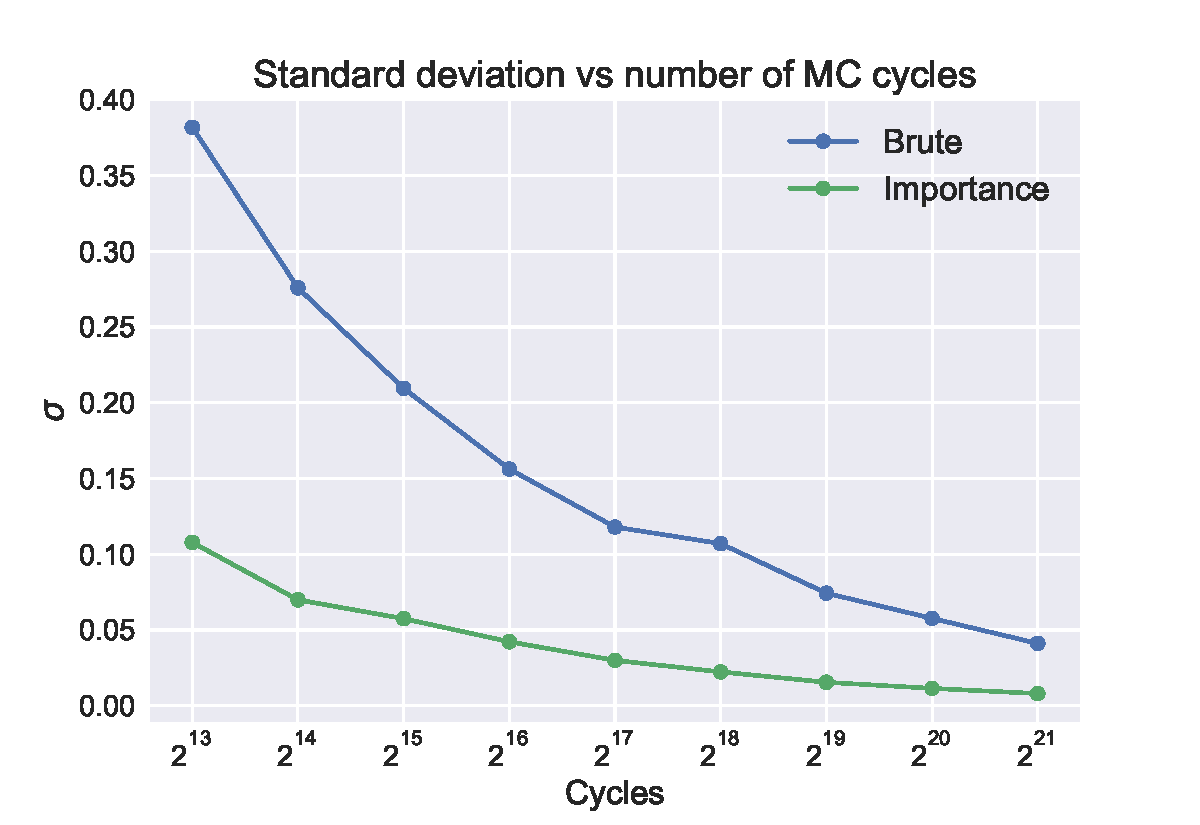
\includegraphics[width=244px]
                    {../data/figures/problem_c1.pdf}
                    \caption{As the number of Monte Carlo cycles increases, the
                    standard deviation of the expectation value of the energy
                    for the brute force and importance sampling schemes
                    decreases.}
                    \label{fig:problem_c1}
            \end{figure}

            \begin{figure}
                \centering
                    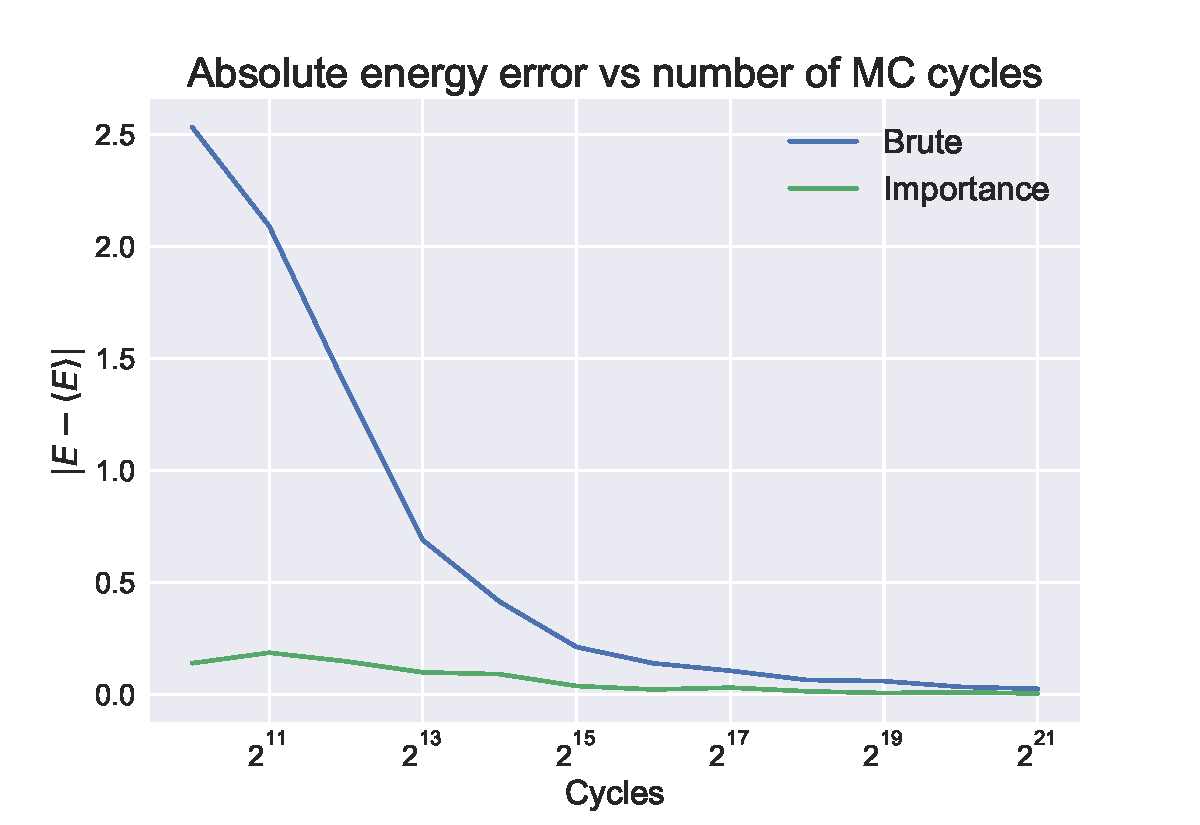
\includegraphics[width=244px]
                    {../data/figures/problem_c2.pdf}
                    \caption{The absolute difference between the expected energy
                    and the exact energy for both the brute force method and
                    importance sampling.}
                    \label{fig:problem_c2}
            \end{figure}

            In \autoref{fig:problem_c1} we can see the standard deviation of the
            local energies for an increasing number of Monte Carlo cycles for
            both the brute force sampling and the importance sampling methods.
            We see that the standard deviation decreases for both methods for a
            larger number of Monte Carlo cycles, but the standard deviation is
            always lower for the importance sampling method. This is in
            accordance with our expectations.

            We have also compared the expected energy with the exact energy for
            a different number of Monte Carlo cycles. The result of this
            analysis is shown in \autoref{fig:problem_c2}. We see that both
            methods will eventually result in expected energies that are equal
            to the exact energies as $\abs{E - \expval{E}} \to 0$. However, for
            the method of importance sampling the error is consistently lower.

            \begin{table}
                \caption{Importance sampled simulations of $N=10$ particles in
                $d=3$ dimensions. Average acceptance ratios and standard
                deviations for eleven values of $\alpha \in [0.3, 0.7]$.}
                \centering
                    \begin{ruledtabular}
                        \begin{tabular}{cccc}
                            $\delta t$ & $\bar{\sigma}_b$ & $\bar{A}$
                            & $\expval{E}\left(\alpha = 1/2\right)$ \\
                            \hline
                            $2^{+3}$ & 0.09363 & 0.005 & 15.000 \\
                            $2^{+2}$ & 0.01549  & 0.041 & 15.000 \\
                            $2^{+1}$ & 0.00706 & 0.216 & 15.000 \\
                            $2^{\ 0}$ & 0.00675 & 0.510 & 15.000 \\
                            $2^{-1}$ & 0.00932 & 0.738 & 15.000 \\
                            $2^{-2}$ & 0.01578 & 0.866 & 15.000 \\
                            $2^{-3}$ & 0.02723 & 0.933 & 15.000 \\
                            $2^{-4}$ & 0.05016 & 0.966 & 15.000 \\
                            $2^{-5}$ & 0.08474 & 0.983 & 15.000 \\
                            $2^{-6}$ & 0.11555 & 0.992 & 15.000 \\
                            $2^{-7}$ & 0.17070 & 0.996 & 15.000 \\
                        \end{tabular}
                    \end{ruledtabular}
                    \label{tab:imp_time_step}
            \end{table}

            \autoref{tab:imp_time_step} shows the standard deviations and
            acceptance ratios for different time steps, $\delta t$ using the
            importance sampling method. The simulations in this table are from
            the same values of $\alpha$ as in \autoref{tab:1D1N_analytic} and
            \autoref{tab:1D1N_numeric}. The optimum energies for $\alpha = 1/2$
            gives the same result for importance sampling as for the naïve way
            of sampling. Notice that by lowering $\delta t$, the uncertainty
            starts to decrease and then starts to increase again. Moreover, the
            acceptance ratios increases as $\delta t \to 0$. This happens as the
            change in the wavefunction grows minuscule and $q(\vf{r}_{i + 1},
            \vf{r}_i) \approx 1$.

    \subsection{Interacting elliptical harmonic oscillator}
        We now make a change to the simple system in the previous section in
        order to make everything a bit more interesting. The potential in the
        one-body Hamiltonian is perturbed in the $z$-direction according to
        \autoref{eq:scaled_hamiltonian} by setting $\lambda = \sqrt{8} \approx
        2.82843$. This corresponds to enclosing particles of the simulation in
        an elliptical trap instead of a spherical trap.

        We also choose a new trial wavefunction with the elliptical gaussian
        single particle functions and the Jastrow factor. The hard sphere radius
        is set to $a = 0.0043$.

        Due to similarities with the spherical harmonic oscillator
        system we make a guess that the true minimum of this new system should
        be situated close to the minimum of the previous system. Choosing seven
        values for $\alpha \in [0.2, 0.7]$ we run importance sampling on this
        system for $N = \{10, 50, 100\}$ particles in $d = 3$ dimensions using
        $2^{21}$ Monte Carlo cycles\footnote{This turned out to be a little bit
        overkill due to the fast convergence of importance sampling.} and an
        additional $10\%$ of the Monte Carlo cycles for thermalization of the
        system prior to doing any sampling. We have used $\delta t = 0.1$ which
        yields a high acceptance ratio, but slower convergence.

        In \autoref{tab:10_interacting} the system is set to have $N = 10$
        interacting particles. Notice first that the energy is higher in
        the interacting system than for a comparable non-interacting system
        (\autoref{tab:initial_optimum_comparison}).  Moreover, the standard
        deviation gets lower as the system is close to an optimal variational
        parameter.

        \begin{table}
            \caption{Simulation results for $N = 10$ bosonic interacting,
            elliptical, harmonic oscillators.}
            \centering
            \begin{ruledtabular}
                \begin{tabular}{ccccc}
                    $\alpha$ & $\langle  E_L\rangle$ & $\sigma_b$
                    &$A$ & $t_{\text{CPU}} [\si{\second}]$ \\
                    \hline
                    0.2&35.17548&0.05399&0.990%98995
                    &24.5\\%48868\\
                    0.3&27.62004&0.02311&0.981%98187
                    &13.6\\%65132\\
                    0.4&24.97850&0.00827&0.972%97248
                    &13.5\\%54666\\
                    0.5&24.39877&0.00030&0.961%96140
                    &13.4\\%38388\\
                    0.6&24.83863&0.00604&0.950%94998
                    &13.3\\%31570\\
                    0.7&25.82855&0.01059&0.938%93766
                    &13.2\\%20579\\
                    0.8&27.22895&0.01436&0.924%92375
                    &13.1\\%11933\\
                \end{tabular}
            \end{ruledtabular}
            \label{tab:10_interacting}
        \end{table}

        The result of simulations with a higher number of particles, $N=50$ and
        $N=100$, are  shown in \autoref{tab:50_interacting} and
        \autoref{tab:100_interacting} respectively. We observe that the energy
        for systems of interacting particles increases rapidly with the size of
        the system.

        \begin{table}
            \caption{Simulation results for $N = 50$ bosonic interacting,
            elliptical, harmonic oscillators.}
            \centering
            \begin{ruledtabular}
                \begin{tabular}{ccccc}
                    $\alpha$ & $\langle  E_L\rangle$ & $\sigma_b$
                    & $A$ & $t_{\text{CPU}} [\si{\second}]$ \\
                    \hline
                    0.2&181.69371&0.25533&0.987%98756
                    &199.9\\%95366\\
                    0.3&142.61591&0.10782&0.978%97849
                    &195.8\\%80928\\
                    0.4&129.88615&0.04051&0.969%96862
                    &190.4\\%44553\\
                    0.5&127.29926&0.00595&0.957%95749
                    &195.1\\%10368\\
                    0.6&129.97630&0.03300&0.946%94595
                    &193.2\\%22755\\
                    0.7&135.67382&0.05785&0.933%93330
                    &192.0\\%191.96391\\
                    0.8&143.23238&0.07286&0.921%92061
                    &192.7\\%72399\\
                \end{tabular}
            \end{ruledtabular}
            \label{tab:50_interacting}
        \end{table}

        \begin{table}
            \caption{Simulation results for $N = 100$ bosonic interacting,
            elliptical, harmonic oscillators.}
            \centering
            \begin{ruledtabular}
                \begin{tabular}{ccccc}
                    $\alpha$ & $\langle  E_L\rangle$ & $\sigma_b$
                    &$A$ & $t_{\text{CPU}} [\si{\second}]$ \\
                    \hline
                    0.2&375.04401&0.51475&0.985%98527
                    &745.2\\%21438\\
                    0.3&296.76879&0.20214&0.975%97534
                    &741.0\\%04425\\
                    0.4&270.60830&0.08113&0.945%94522
                    &723.1\\%06823\\
                    0.5&266.37263&0.02020&0.953%95314
                    &702.8\\%71000\\
                    0.6&272.51171&0.07366&0.941%94112
                    &689.1\\%12862\\
                    0.7&285.10285&0.11381&0.929%92895
                    &707.5\\%48248\\
                    0.8&301.40609&0.15458&0.916%91648
                    &707.9\\%86118\\
                \end{tabular}
            \end{ruledtabular}
            \label{tab:100_interacting}
        \end{table}

        \subsubsection{Finding the minimum}
            Using the method of gradient descent we choose a set of six starting
            $\alpha_0 \in [0.2, 0.8]$ and try to locate a value for $\alpha$
            where the gradient goes to zero. We looked at $N = 10$ with $d = 3$,
            $\omega = 1$ and $\beta = \lambda = \sqrt{8}$. This yields the value
            for the minimum $\alpha$ to be
            \begin{align}
                \alpha = 0.49744 \pm 0.00002.
                \label{eq:optimal_interacting_alpha}
            \end{align}
            In \autoref{fig:gradient_descent_interacting} we can see how the
            conjugate gradient method "moves" to find the optimal value of
            $\alpha$.

            For this value of $\alpha$ we have computed the expected energy and
            standard deviation for systems of $N = \{10, 50, 100\}$ particles.
            These results are shown in \autoref{tab:interacting_optimal}. We have
            compared with the non-interacting case, i.e., where the Jastrow
            factor is zero ($a = 0$).

            \begin{figure}
                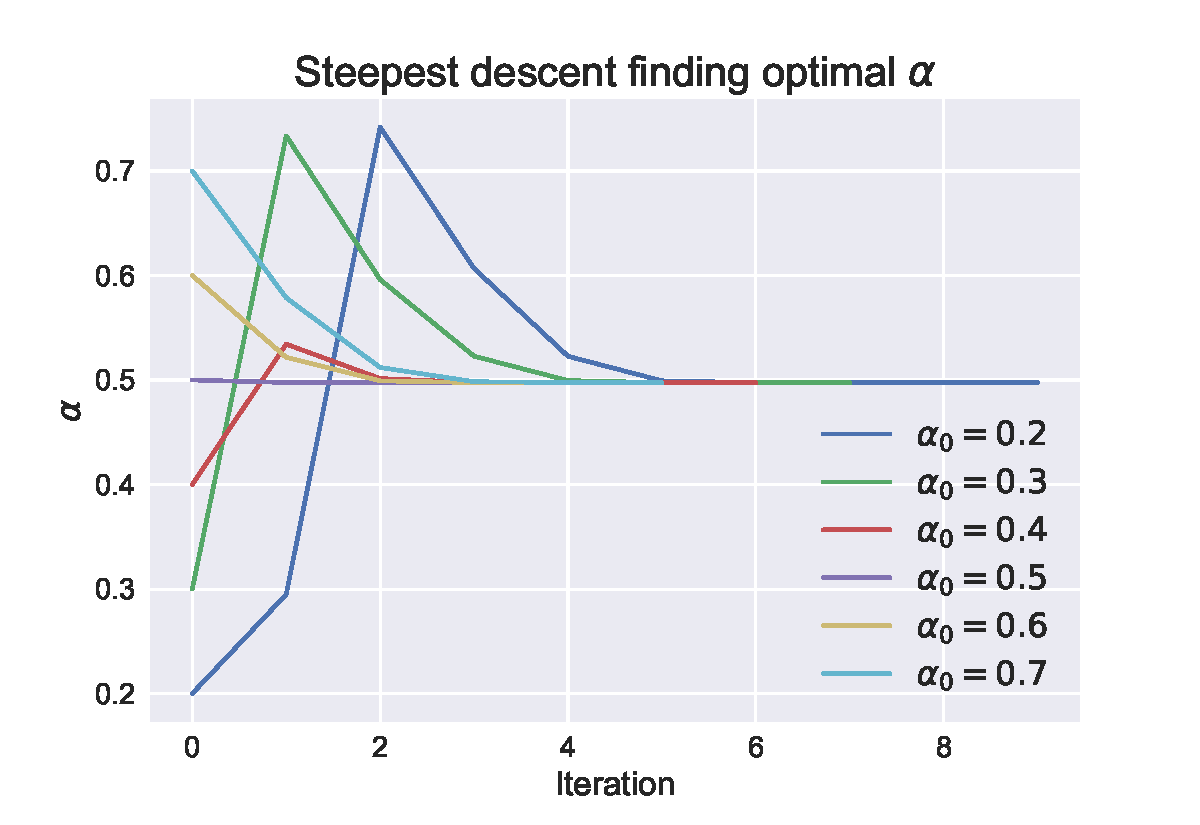
\includegraphics[width=244px]{../data/figures/problem_f.pdf}
                \caption{In this figure we can see the convergence of different
                starting values for $\alpha$ towards the true value of $\alpha$
                that minimizes the expected energy in the interacting case.}
                \label{fig:gradient_descent_interacting}
            \end{figure}

            \begin{table}
                \caption{Comparison of an elliptical gaussian trial wavefunction
                with and without the Jastrow factor using the elliptical trap.}
                \centering
                \begin{ruledtabular}
                    \begin{tabular}{r|rr|rr}
                        & \multicolumn{2}{c|}{Interacting}
                        & \multicolumn{2}{c}{Non-interacting} \\
                        \hline
                        $N$ & $\expval{E}$ & $\sigma_b$ & $\expval{E}$
                        & $\sigma_b$ \\
                        \hline
                        10 & 24.3986 & 0.0003 & 24.1418 & 0.0002 \\
                        50 & 127.2852 & 0.0077 & 120.7129 & 0.0012 \\
                        100 & 266.2904 & 0.0297 & 241.4248 & 0.0025
                    \end{tabular}
                \end{ruledtabular}
                \label{tab:interacting_optimal}
            \end{table}

        \subsubsection{One-Body Densities}
            We now look at one-body densities for the value of $\alpha$ found in
            \autoref{eq:optimal_interacting_alpha}. The results for a system
            consisting of $N=100$ particles are displayed in
            \autoref{fig:one_body_density_100}.  In this figure we see the
            densities for a system confined to a perturbed elliptic trap with
            and without interaction. We see that for the interacting case, the
            one-body density is skewed towards a larger $\abs{\vf{r}}$, as is
            expected. The hard core prevents the bosons from stacking on top of
            each other spatially. By increasing the hard core radius this trend
            will be more noticeable. The one-body density of the "ideal" system
            is also included in the figure.


            \begin{figure}
                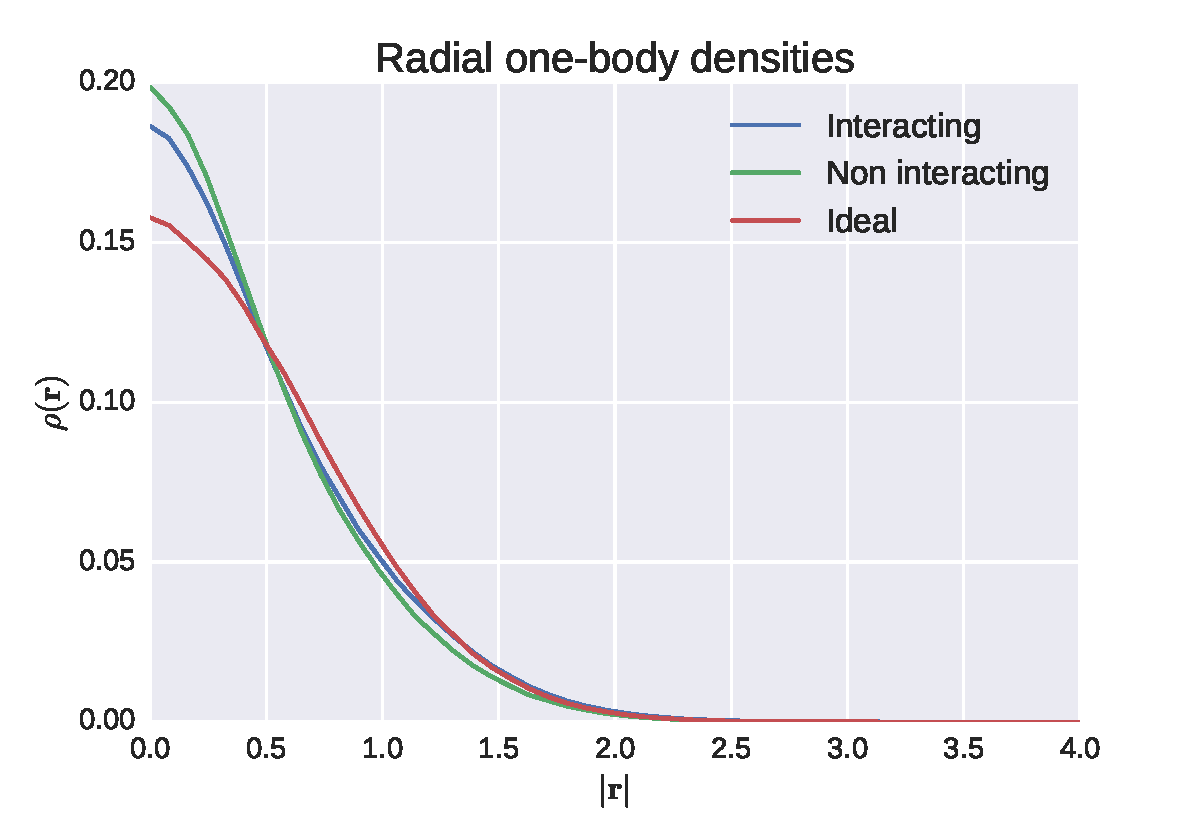
\includegraphics[width=244px]
                {../data/figures/problem_g_100N.pdf}
                \caption{In this figure the interacting and non-interacting
                densities correspond to the elliptical potential with and
                without the Jastrow factor respectively. The "ideal" system is
                the spherical potential with the non-interacting Gaussian trial
                wavefunction.}
                \label{fig:one_body_density_100}
            \end{figure}


\section{Discussion}

    \subsection{Validity of Results}
        The non-interacting tests compared against the analytic "solution"
        showed to a very high degree the validity of the method. One can see
        this quite clearly from \autoref{fig:initial_problem_b}. Because we get
        results from simulations that correspond to the analytic results we can
        be fairly certain that the method can be expanded upon to include
        attributes outside the realm of problems that are analytically solvable.
        The systems with the elliptic traps and the interacting particles have
        just such attributes.

        That said, the way to get the best confirmation of the results presented
        above is in comparison to experiment. This would be quite difficult
        as the systems presented are very theoretical in nature and most likely
        far from anything we would see in nature. Without being able to compare
        our result with anything happening in the real world this entire study would
        have no value except for the instrumental value, being no more than
        a theoretical exercise.  However, the one-body
        density is a measure of the role of many-body correlations which in
        some cases can be related to experiment. For a system of charged
        particles it can be used to determine a charge distribution, which in
        turn can be linked to experiment. It would be very fruitful to simulate a
        system of such particles that is more natural, i.e. real, but we realise the
        purpose of this study is first and foremost to introduce variational
        Monte Carlo as a tool in computational physics. We assume, however, that
        this study is a good starting point for studies of alkali atoms like
        $^{87}$Rb, $^{23}$Na or $^7Li$.

    \subsection{Energy per particle}
        For the non-interacting harmonic oscillator system there is no
        difference between a new particle and a new dimension\footnote{This is
        not entirely true in the case of our implementation of the
        Metropolis-Hastings algorithm as we draw a single random particle and
        move all dimensions instead of iterating over all particles and all
        dimensions.}. This means that the inclusion of a new particle or
        dimension yields a linear scaling in the energy. Thus if we compute the
        energy per particle for systems of varying size we expect to get the
        same energy. This is most easily seen in \autoref{fig:initial_problem_b}
        and in the expression for the exact energy \autoref{eq:exact_energy}.

        This, however, is \emph{not} the case in the interacting system due to
        the Jastrow factor. Looking at \autoref{tab:10_interacting} and
        \autoref{tab:100_interacting} we see that multiplying the expected
        energy of the former with $10$ yields a lower number than the latter. We
        can also see this behavior in \autoref{fig:interacting}, where the
        energy per particle for $N = \{10, 50, 100\}$ have been plotted in the
        same figure.

        \begin{figure}
            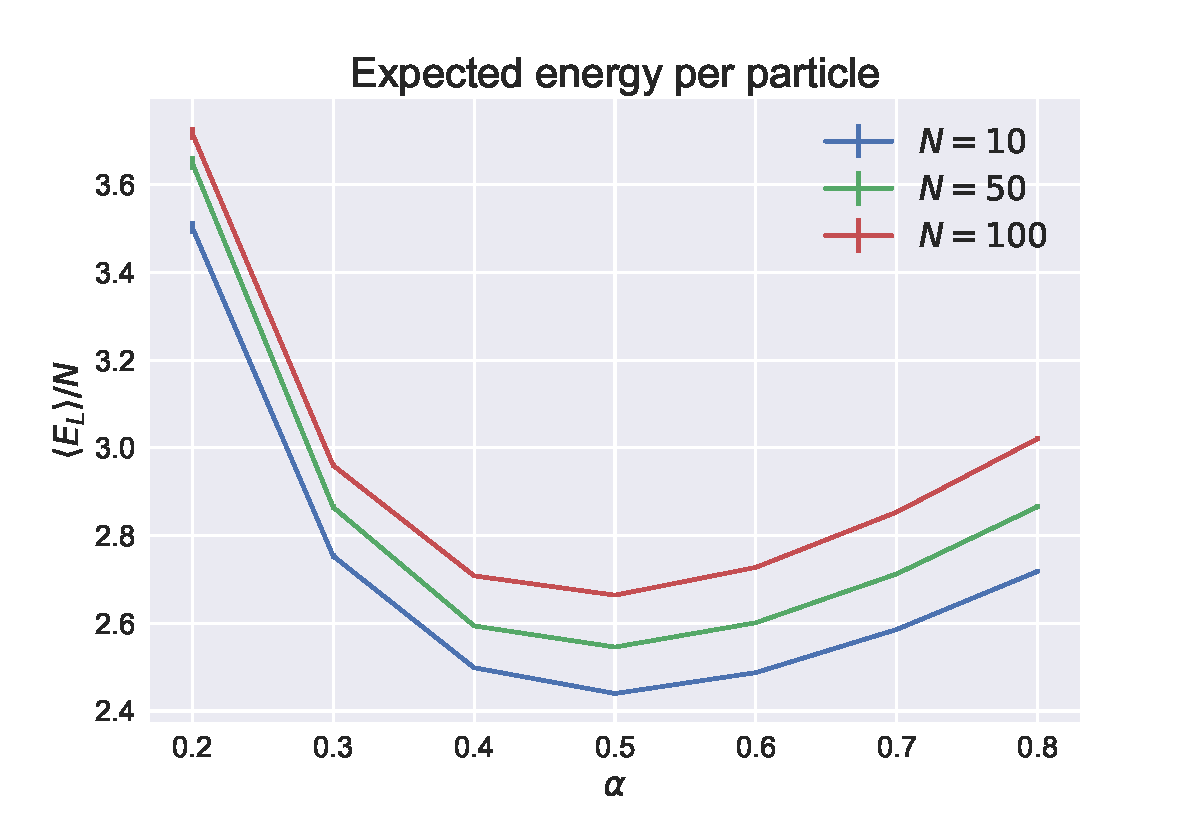
\includegraphics[width=244px]{../data/figures/problem_e.pdf}
            \caption{Expected energy per particle as a function of variational
            parameter $\alpha$ for a varying number of particles.}
            \label{fig:interacting}
        \end{figure}

        The reason for the increase in energy per particle can be ascribed to
        the repulsive interaction added by the Jastrow factor. The repulsive
        force can be explained thusly: the Jastrow factor  increases the value
        of the local energy for any given particle if that particle is some
        distance away from any other particle. The closer the particles are, the
        more the local energy increases. The Jastrow factor will lower the
        probability for the particles to get too close to one another by
        reducing the probability density in the vicinity of other particles.
        However, if there are many particles in the system they will be closer
        to another particle and therefore increase the energy of the system.

    \subsection{Low density system}
        It is safe to say that the effect of adding a Jastrow factor is significant,
        i.e. the increase in
            energy for the system as the interaction is switched on is much higher
            than the uncertainty of the energy. A simple look at \autoref{fig:interacting}
            will be proof enough as the error bars of the figure are not discernible.
        On the other hand, the energy added to the system by including interaction
        is not very high compared to the energy of the system as a whole. For the
        larger of the interacting systems we have looked at, with $n=100$ particles,
        The interaction add only a mere $9\%$ extra energy (see \autoref{tab:interacting_optimal}).
        Studying \autoref{fig:one_body_density_100} will reveal the same.

        The reason for this stems from the assumption which justifies that
        adding only two-body interaction is sufficient to model all interaction to a
        reasonable extent. This assumption is justified by the fact that alkali and
        atomic hydrogen systems\footnote{Systems similar to our toy model}
        are dilute. For gases of alkali atoms confined in magnetic or optical traps
        the average distance between atoms is much larger than the range of
        inter-atomic interaction. The probability is high that atoms very seldom
        interact and if so, just with one other atom.

\section{Summary Remarks}

    In this study we have built a functional variational Monte Carlo solver framework for
    a gas following Bose-Einstein statistics confined in an elliptic trap. Monte Carlo
    methods is a broad class of computational algorithms, whereas the variational
    Monte Carlo is a subset. Other applications of such methods within the physical
    sciences includes, but is not limited to, quantum chromodynamics, the modeling of
    aearodynamic forms, particle physics detector design and galaxy evolution.
    Needless to say, Monte Carlo method is a valuable tool for a computational physicist.

    To prove the
    validity of the framework we tested it against an analytically solved case, an ideal
    non-interacting system. Thereafter we have shown how our implementation can
    handle large systems of interacting particles and perturbed traps. Even though
    this study is somewhat theoretic in nature, we have discussed the possibility of
    expanding our machinery to a case bearing a larger resemblance to a system
    found in nature. To this end we have computed one-body densities for the
    interacting system, which can be compared to real physical properties as
    measured in an experiment.


\bibliography{references}
\clearpage

\appendix
\section{Computing the exact energy of the non-interacting system}
    Here we show how to arrive at \autoref{eq:exact_energy}. We need to solve
    two integrals consisting of $N$, $d$-dimensional, Gaussians from
    \autoref{eq:trial_simple_gaussian}. We will label the position in the $j$-th
    coordinate for the $i$-th particle by $x_{ij}$. Starting with the
    normalization factor we get
    \begin{align}
        \bra{\Psi_T}\ket{\Psi_T}
        &=
        \int\dd\vf{r}\abs{\Psi_T(\vf{r})}^2
        \\
        &=
        \prod_{i = 1}^N
        \int\dd\vf{r}_i\exp(-2\alpha\vf{r}_i^2)
        \\
        &=
        \prod_{i = 1}^N
        \prod_{j = 1}^d
        \int\dd x_{ij}\exp(-2\alpha x_{ij}^2)
        \\
        &=
        \prod_{i = 1}^N
        \prod_{j = 1}^d
        \sqrt{\frac{\pi}{2\alpha}}
        = \para{
            \sqrt{\frac{\pi}{2\alpha}}
        }^{dN}.
    \end{align}
    From the Hamiltonian we get two integrals containing $\vf{r}_i^2$ for each
    particle $i$.
    \begin{align}
        \bra{\Psi_T}\vf{r}_i^2\ket{\Psi_T}
        &=
        \int\dd\vf{r}\abs{\Psi_T(\vf{r})}^2\vf{r}_i^2
        \\
        &=
        \int\dd\vf{r}_i\exp(-2\alpha\vf{r}_i^2)\vf{r}_i^2
        \nonumber \\
        &\qquad
        \times
        \prod_{j \neq i}^N
        \int\dd\vf{r}_j\exp(-2\alpha\vf{r}_j^2)
        \\
        &=
        \sum_{l = 1}^d
        \int
        \para{
            \prod_{k = 1}^d
            \dd x_{ik}\exp(-2\alpha x_{ik}^2)
        } x_{il}^2
        \nonumber\\
        &\qquad
        \times
        \para{
            \sqrt{\frac{\pi}{2\alpha}}
        }^{d(N - 1)}
        \\
        &=
        \sum_{l = 1}^d
        \frac{1}{4\alpha}\sqrt{\frac{\pi}{2\alpha}}
        \para{
            \sqrt{\frac{\pi}{2\alpha}}
        }^{d - 1}
        \nonumber\\
        &\qquad
        \times
        \para{
            \sqrt{\frac{\pi}{2\alpha}}
        }^{d(N - 1)}
        \\
        &= \frac{d}{4\alpha}\para{
            \sqrt{\frac{\pi}{2\alpha}}
        }^{dN}.
    \end{align}
    We thus have that
    \begin{align}
        \frac{\bra{\Psi_T}\vf{r}_i^2\ket{\Psi_T}}{\bra{\Psi_T}\ket{\Psi_T}}
        &=
        \frac{d}{4\alpha}.
    \end{align}
    Using \autoref{eq:laplacian_simple_gaussian} we can find the exact energy
    expression we are looking for.
    \begin{align}
        E(\alpha)
        &=
        \frac{\bra{\Psi_T}H\ket{\Psi_T}}{\bra{\Psi_T}\ket{\Psi_T}}
        \\
        &=
        \sum_{i = 1}^N
        \brac{
            -\frac{\hbar^2}{2m}
            \brak{
                -2d\alpha
                + 4\alpha^2\frac{d}{4\alpha}
            }
            + \frac{1}{2}m\omega^2\frac{d}{4\alpha}
        }
        \\
        &=
        \para{
            \frac{\alpha\hbar^2}{2m}
            + \frac{m\omega^2}{8\alpha}
        }dN,
    \end{align}
    which is what we wanted to show.


\section{Computing the drift force and local energy of the full system}
    Computing the gradient of the wavefunction we get
    \begin{align}
        \nabla_k\Psi_T(\vf{r})
        &=
        \Bigl[
            \nabla_k
            \Phi_T(\vf{r})
        \Bigr]
        J(\vf{r})
        + \Phi_T(\vf{r})
        \nabla_k J(\vf{r}).
    \end{align}
    The gradient of the Slater permament for particle $k$ is given by
    \begin{align}
        \nabla_k
        \Phi_T(\vf{r})
        &=
        \nabla_k\phi_k
        \prod_{i \neq k}^N\phi_i
        = \frac{\nabla_k\phi_k}{\phi_k}
        \Phi_T(\vf{r}).
    \end{align}
    The gradient of the Jastrow factor is given by
    \begin{align}
        \nabla_k J(\vf{r})
        &=
        J(\vf{r})
        \nabla_k\sum_{m < n}^N u_{mn} \\
        &= J(\vf{r})
        \Biggl(
            \sum_{m = 1}^{k - 1}\nabla_k u_{mk}
            \sum_{n = k + 1}^N\nabla_k u_{kn}
        \Biggr)
        \\
        &=
        J(\vf{r})
        \sum_{m \neq k}^N\nabla_k u_{km},
    \end{align}
    where the gradient of the interaction term splits the antisymmetric
    sum into two parts. As $r_{ij} = r_{ji}$ we can combine these sums
    into a single sum. This in total yields the gradient
    \begin{align}
        \nabla_k\Psi_T(\vf{r})
        &=
        \Biggl(
            \frac{\nabla_k\phi_k}{\phi_k}
            + \sum_{m \neq k}^N
            \nabla_k u_{km}
        \Biggr)
        \Psi_T(\vf{r}).
        \label{eq:gradient_full_wavefunction}
    \end{align}

    The Laplacian of the trial wavefunction is found by finding the
    divergence of \autoref{eq:gradient_full_wavefunction}.
    \begin{align}
        \nabla_k^2\Psi_T(\vf{r})
        &=
        \Biggl(
            \nabla_k\Biggl[
                \frac{\nabla_k\phi_k}{\phi_k}
            \Biggr]
            +
            \sum_{m \neq k}^N \nabla_k^2 u_{km}
        \Biggr)\Psi_T(\vf{r})
        \\
        &\qquad
        +
        \Biggl(
            \frac{\nabla_k\phi_k}{\phi_k}
            + \sum_{m \neq k}^N
            \nabla_k u_{km}
        \Biggr)^2
        \Psi_T(\vf{r}),
    \end{align}
    where the squared term came from taking the gradient of the trial
    wavefunction.  To further simplify we divide by the trial
    wavefunction. This yields
    \begin{align}
        \frac{\nabla_k^2\Psi_T(\vf{r})}{\Psi_T(\vf{r})}
        &=
        \frac{\nabla_k^2\phi_k}{\phi_k}
        + 2\frac{\nabla_k\phi_k}{\phi_k}
        \sum_{m \neq k}\nabla_k u_{km}
        \nonumber \\
        &\qquad
        + \sum_{m\neq k}^N\nabla_k^2 u_{km}
        + \Biggl(
            \sum_{m \neq k}^N\nabla_k u_{km}
        \Biggr)^2.
    \end{align}
    From here, the next step is to find the gradient and the Laplacian of
    the single particle functions, $\phi_k$, and the interaction
    functions $u_{km}$. For the single particle functions we use
    Cartesian coordinates when finding the derivatives while for
    the interaction functions we use spherical coordinates and do a
    variable substitution. Beginning with the gradient of the single
    particle functions we get
    \begin{align}
        \nabla_k\phi_k
        &=
        \nabla_k\exp\bigl[
            -\alpha(x_k^2 + y_k^2 + \beta z_k^2)
        \bigr] \\
        &=
        -2\alpha
        (x_k\vf{e}_i + y_k\vf{e}_j + \beta z_k\vf{e}_k)
        \phi_k.
    \end{align}
    Note that the subscripts on the unit vectors $\vf{e}_i$ are
    \emph{not} the same as the subscripts used for its components. The
    Laplacian yields
    \begin{align}
        \nabla_k^2\phi_k
        &=
        \Bigl[
            -2\alpha
            \big(
                d - 1 + \beta
            \bigr)
            \nonumber \\
            &\qquad
            + 4\alpha^2
            \bigl(
                x_k^2 + y_k^2 + \beta^2z_k^2
            \bigr)
        \Bigr]
        \phi_k,
    \end{align}
    with $d$ as the dimensionality of the problem.
    In order to derive the interaction functions we have to do a
    variable substitution using $r_{km} = |\vf{r}_k - \vf{r}_m|$. We can
    then rewrite the $\nabla_k$-operator as
    \begin{align}
        \nabla_k
        &=
        \nabla_k
        \dpd[]{r_{km}}{r_{km}}
        =
        \nabla_k r_{km} \dpd[]{}{r_{km}}
        \\
        &=
        \frac{\vf{r}_k - \vf{r}_m}{r_{km}}\dpd[]{}{r_{km}}.
    \end{align}
    Applying this version of the $\nabla_k$-operator to $u_{km}$ yields
    \begin{align}
        \nabla_k u_{km}
        &=
        \frac{\vf{r}_k - \vf{r}_m}{r_{km}}
        \dpd[]{u_{km}}{r_{km}}.
    \end{align}

    \begin{widetext}
        For the Laplacian we switch a little back and forth between the
        two ways of representing the $\nabla_k$-operator. We thus get
        \begin{align}
            \nabla_k^2 u_{km}
            &=
            \frac{\nabla_k \vf{r}_k}{r_{km}}\dpd[]{u_{km}}{r_{km}}
            + \Biggl[
                \nabla_k \frac{1}{r_{km}}
            \Biggr]
            (\vf{r}_k - \vf{r}_m)\dpd[]{u_{km}}{r_{km}}
            + \frac{\vf{r}_k - \vf{r}_m}{r_{km}}
            \nabla_k \dpd[]{u_{km}}{r_{km}} \\
            &= \frac{d}{r_{km}}\dpd[]{u_{km}}{r_{km}}
            - \frac{(\vf{r}_k - \vf{r}_m)^2}{r_{km}^3}
            \dpd[]{u_{km}}{r_{km}}
            + \frac{(\vf{r}_k - \vf{r}_m)^2}{r_{km}^2}
            \dpd[2]{u_{km}}{r_{km}} \\
            &=
            \frac{d - 1}{r_{km}}\dpd[]{u_{km}}{r_{km}}
            + \dpd[2]{u_{km}}{r_{km}},
        \end{align}
        where $d$ is again the dimensionality of the problem. In total
        we can state an intermediate version of the Laplacian occuring
        in the local energy as
        \begin{align}
            \frac{\nabla_k^2\Psi_T(\vf{r})}{\Psi_T(\vf{r})}
            &=
            \frac{\nabla_k^2\phi_k}{\phi_k}
            + 2\frac{\nabla_k\phi_k}{\phi_k}
            \sum_{m \neq k}^N
            \frac{\vf{r}_k - \vf{r}_m}{r_{km}}
            \dpd[]{u_{km}}{r_{km}}
            + \sum_{m\neq k}^N
            \Biggl(
                \frac{d - 1}{r_{km}}\dpd[]{u_{km}}{r_{km}}
                + \dpd[2]{u_{km}}{r_{km}}
            \Biggr)
            \nonumber \\
            &\qquad
            +
            \sum_{m, n \neq k}^N
            \frac{\vf{r}_k - \vf{r}_m}{r_{km}}
            \frac{\vf{r}_k - \vf{r}_n}{r_{kn}}
            \dpd[]{u_{km}}{r_{km}}
            \dpd[]{u_{kn}}{r_{kn}}.
        \end{align}
    \end{widetext}
    Moving on to the derivatives of the interaction terms, $u_{km}$, to
    get an explicit expression for the Laplacian.
    \begin{align}
        \dpd[]{u_{km}}{r_{km}}
        &=
        \frac{a}{r_{km}(r_{km} - a)},
        \\
        \dpd[2]{u_{km}}{r_{km}}
        &= \frac{a^2 - 2ar_{km}}{r_{km}^2(r_{km} - a)^2}.
    \end{align}
    The local energy and the drift force can now be found by combining these
    expressions. We will not write out the explicit expressions as
    these will be called by separated functions in our programs.


\section{Variational parameter gradient of the expectation energy}
    Here we show how to arrive at the expression shown in
    \autoref{eq:variational_parameter_gradient}. This requires us to restrict
    our view to real trial wavefunctions, i.e., $\Psi_T^{*} = \Psi_T$, which is
    the case for the wavefunctions we are exploring.
    \begin{align}
        \nabla_{\vfg{\alpha}}\expval{E_L}
        &=
        \nabla_{\vfg{\alpha}}
        \para{
            \frac{
                \int\dd\vf{r}\Psi_T^{*}H\Psi_T
            }{
                \int\dd\vf{r}|\Psi_T|^2
            }
        }
        \\
        &=
        -
        \frac{
            2
            \para{
                \int\dd\vf{r}\Psi_T H\Psi_T
            }
        }{\para{\int\dd\vf{r}\Psi_T}^2}
        \int\dd\vf{r}\Psi_T\nabla_{\vfg{\alpha}}\Psi_T
        \\
        &\qquad
        +
        \frac{2}{\int\dd\vf{r}\Psi_T^2}
        \int\dd\vf{r}\Psi_TH\brak{
            \nabla_{\vfg{\alpha}}\Psi_T
        }
        \\
        &=
        - 2\expval{E_L}
        \frac{1}{
            \int\dd\vf{r}\Psi_T^2
        }
        \int\dd\vf{r}\Psi_T^2\para{
            \frac{\nabla_{\vfg{\alpha}}\Psi_T}{\Psi_T}
        }
        \\
        &\qquad
        +
        \frac{2}{\int\dd\vf{r}\Psi_T^2}
        \int\dd\vf{r}\Psi_T^2 E_L\para{
            \frac{\nabla_{\vfg{\alpha}}\Psi_T}{\Psi_T}
        }.
    \end{align}
    We now use the definition of the expectation value to group terms together.
    We are thus left with
    \begin{align}
        \nabla_{\vfg{\alpha}}\expval{E_L}
        =
        2
        \para{
            \expval{
                E_L\frac{1}{\Psi_T}\nabla_{\vfg{\alpha}}\Psi_T
            }
            - \expval{E_L}
            \expval{\frac{1}{\Psi_T}\nabla_{\vfg{\alpha}}\Psi_T}
        },
    \end{align}
    which is what we wanted to show.

\clearpage
\onecolumngrid
\section{Brute Force Metropolis-Hastings}
    In \autoref{fig:initial_problem_b} we see how the expectation value of the
    energy for the analytic and numeric expression of the local energy using
    Monte Carlo sampling matches the exact energy from \autoref{eq:exact_energy}
    for $\alpha \in [0.3, 0.7]$.
    \begin{figure}[b]
        \makebox[\textwidth][c]{
            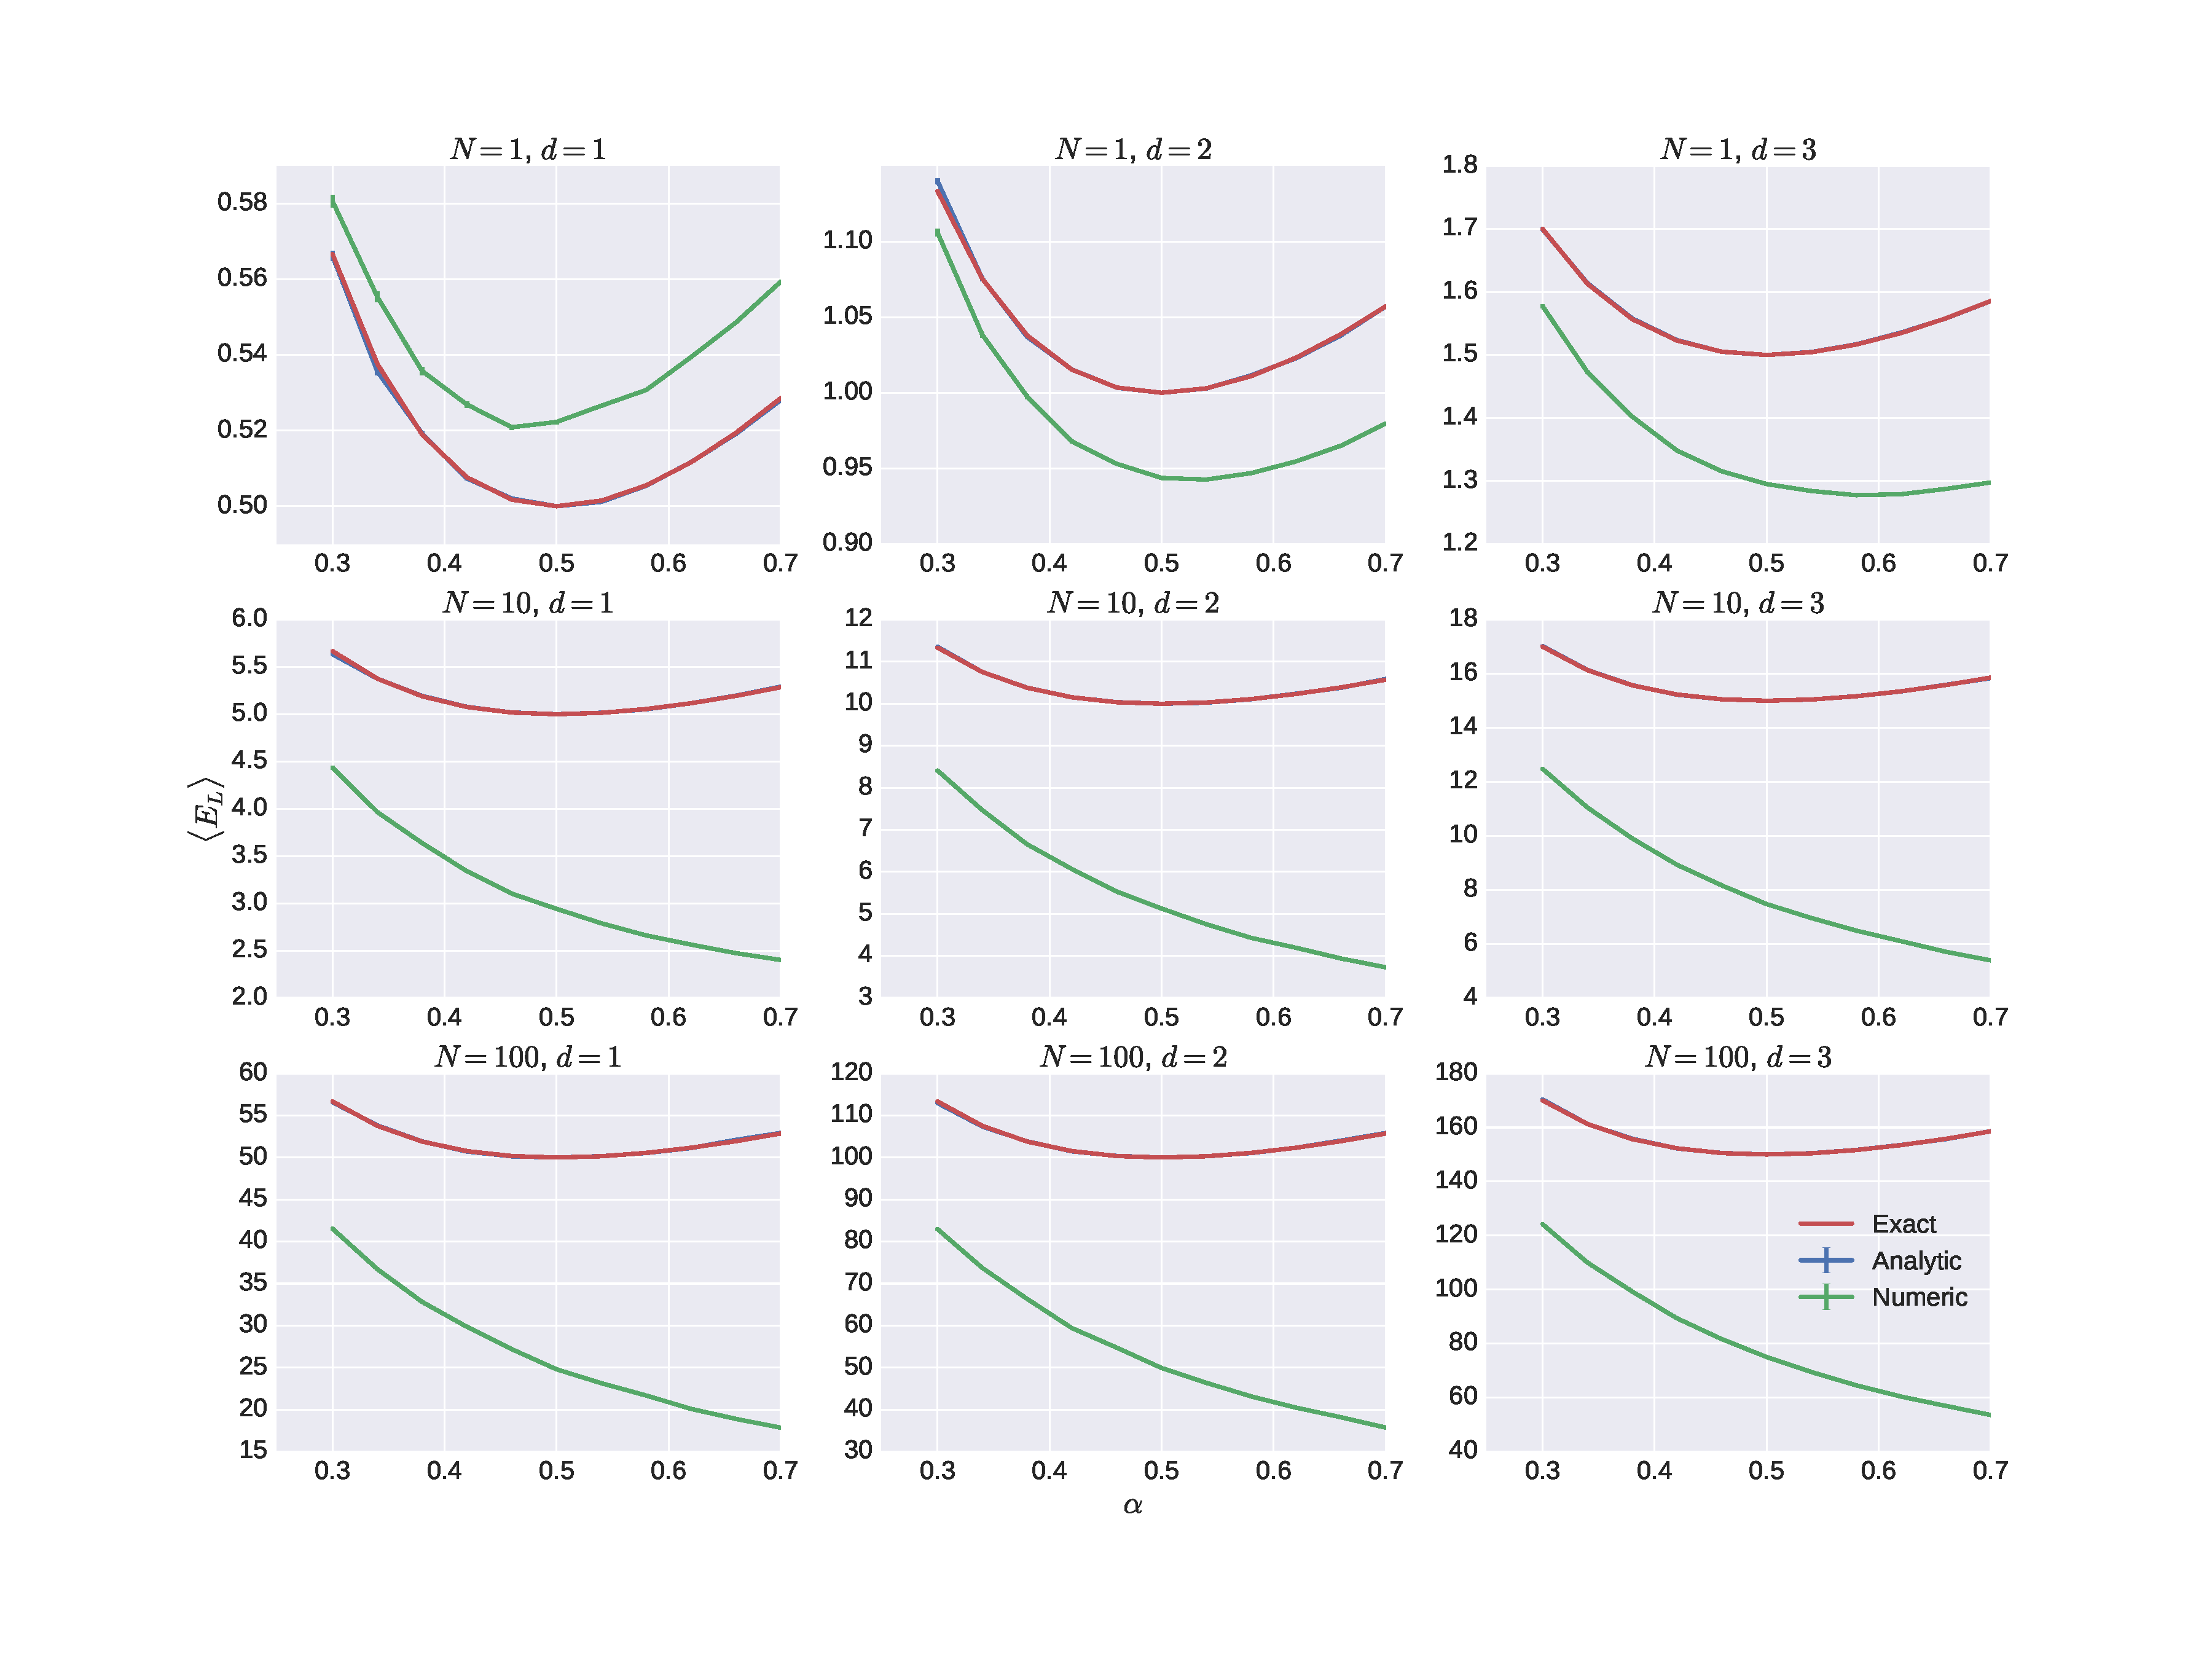
\includegraphics[width=1.2\textwidth]{../data/figures/problem_b.pdf}
        }
        \caption{Comparison of analytic and numeric results with the exact
        expression for the energy as a function of $\alpha$. The plots show the
        standard deviation from the blocking method as error ticks. In the
        figure $N$ is the number of particles and $d$ the number of dimensions.}
        \label{fig:initial_problem_b}
        \vspace{2cm}
    \end{figure}


\end{document}
